%%%%%%%%%%%%%%%%%%%%%%%%%%%%%%%%%%%%%%%%%%%%%%%%%%%%%%%%%%%%%%%%%%%%%%%%%%%%%%%%%%%%%%%%%%%%%%%%%%%%%%%%%%%%%%%%%%%%%%%%%%%%%%%%%%%%%%%%%%%%%%%%%%%%%%%%%%%
% This is just an example/guide for you to refer to when submitting manuscripts to Frontiers, it is not mandatory to use Frontiers .cls files nor frontiers.tex  %
% This will only generate the Manuscript, the final article will be typeset by Frontiers after acceptance.
%                                              %
%                                                                                                                                                         %
% When submitting your files, remember to upload this *tex file, the pdf generated with it, the *bib file (if bibliography is not within the *tex) and all the figures.
%%%%%%%%%%%%%%%%%%%%%%%%%%%%%%%%%%%%%%%%%%%%%%%%%%%%%%%%%%%%%%%%%%%%%%%%%%%%%%%%%%%%%%%%%%%%%%%%%%%%%%%%%%%%%%%%%%%%%%%%%%%%%%%%%%%%%%%%%%%%%%%%%%%%%%%%%%%

%%% Version 3.4 Generated 2018/06/15 %%%
%%% You will need to have the following packages installed: datetime, fmtcount, etoolbox, fcprefix, which are normally inlcuded in WinEdt. %%%
%%% In http://www.ctan.org/ you can find the packages and how to install them, if necessary. %%%
%%%  NB logo1.jpg is required in the path in order to correctly compile front page header %%%

\documentclass[utf8]{frontiersSCNS} % for Science, Engineering and Humanities and Social Sciences articles

\usepackage{url,hyperref,lineno,microtype}
\usepackage{graphicx}
\usepackage{subcaption}
\usepackage[onehalfspacing]{setspace}
\usepackage[english]{babel}
\usepackage[most]{tcolorbox}
\usepackage{tabularx}
% \usepackage[table]{xcolor}    % loads also »colortbl«

\linenumbers

% Leave a blank line between paragraphs instead of using \\

% - Alexander Lalejini - MSU, CSE, BEACON, EEB
% - Austin J. Ferguson - CSE, BEACON, EEB
% - Nkrumah A. Grant - Marx Lab, University of Idaho, Department of Biological Sciences, Moscow, ID, USA, BEACON
% - Charles Ofria - CSE, BEACON, EEB

\def\keyFont{\fontsize{8}{11}\helveticabold }
\def\firstAuthorLast{Lalejini {et~al.}} %use et al only if is more than 1 author
\def\Authors{Alexander Lalejini\,$^{1,2,3,*}$, Austin J. Ferguson\,$^{1,2,3}$, Nkrumah A. Grant\,$^{1,4}$, and Charles Ofria\,$^{1,2,3}$}
% Affiliations should be keyed to the author's name with superscript numbers and be listed as follows: Laboratory, Institute, Department, Organization, City, State abbreviation (USA, Canada, Australia), and Country (without detailed address information such as city zip codes or street names).
% If one of the authors has a change of address, list the new address below the correspondence details using a superscript symbol and use the same symbol to indicate the author in the author list.
% \def\Address{$^{1}$Laboratory X, Institute X, Department X, Organization X, City X , State XX (only USA, Canada and Australia), Country X \\
% $^{2}$Laboratory X, Institute X, Department X, Organization X, City X , State XX (only USA, Canada and Australia), Country X  }
\def\Address{
$^{1}$BEACON Center for the Study of Evolution in Action, Michigan State University, East Lansing, MI, USA \\
$^{2}$Ecology, Evolution, and Behavior Program, Michigan State University, East Lansing, MI, USA \\
$^{3}$Department of Computer Science and Engineering, Michigan State University, East Lansing, MI, USA \\
$^{4}$Department of Biological Sciences, University of Idaho, Moscow, ID, USA
% $^{X}$Laboratory X, Institute X, Department X, Organization X, City X , State XX (only USA, Canada and Australia), Country X \\
% $^{Y}$Laboratory X, Institute X, Department X, Organization X, City X , State XX (only USA, Canada and Australia), Country X
}
% The Corresponding Author should be marked with an asterisk
% Provide the exact contact address (this time including street name and city zip code) and email of the corresponding author
\def\corrAuthor{Alexander Lalejini}

\def\corrEmail{amlalejini@gmail.com}


\begin{document}
\onecolumn
\firstpage{1}

% ============= TITLE IDEAS =============
% - Adaptive phenotypic plasticity stabilizes populations in fluctuating environments
% - The evolution of adaptive phenotypic plasticity stabilizes populations in fluctuating environments
% - Phenotypic plasticity can promote the evolution of complex features in fluctuating environments
% - Adaptive plasticity buffers population against fluctuations, promoting novel trait evolution/retention
% - Phenotypic plasticity can simultaneously slow rate of evolutionary change and promote evo of complex features
% - Phenotypic plasticity can promote the evolution and maintenance of complex features in fluctuating environments
% - Adaptive plasticity stabilizes populations in fluctuating environments and constrains evolutionary outcomes
\title[Adaptive plasticity stabilizes evolution]{Adaptive phenotypic plasticity stabilizes evolution in fluctuating environments}

\author[\firstAuthorLast ]{\Authors} %This field will be automatically populated
\address{} %This field will be automatically populated
\correspondance{} %This field will be automatically populated

\extraAuth{}% If there are more than 1 corresponding author, comment this line and uncomment the next one.
%\extraAuth{corresponding Author2 \\ Laboratory X2, Institute X2, Department X2, Organization X2, Street X2, City X2 , State XX2 (only USA, Canada and Australia), Zip Code2, X2 Country X2, email2@uni2.edu}


\maketitle


%%%%%%%%%%%%%%%%%%%%%%%%%%%%%%%%%%%%
% Utility commands
%%%%%%%%%%%%%%%%%%%%%%%%%%%%%%%%%%%%
\newcommand{\code}{\texttt}


%%%%%%%%%%%%%%%%%%%%%%%%%%%%%%
% Evolutionary change rate experiment
%%%%%%%%%%%%%%%%%%%%%%%%%%%%%%

% data from experiment - 2021-02-08
\newcommand{\evolutionaryChangeRateReplicates}{100}

\newcommand{\evolutionaryChangeRatePlasticReps}{42}


%%%%%%%%%%%%%%%%%%%%%%%%%%%%%%
% Novel traits experiment
%%%%%%%%%%%%%%%%%%%%%%%%%%%%%%
\newcommand{\novelTraitsReplicates}{100}
\newcommand{\novelTraitsReward}{10\%}
\newcommand{\novelTraitsPlasticReps}{42}

%%%%%%%%%%%%%%%%%%%%%%%%%%%%%%
% Deleterious hitchhiking experiment
%%%%%%%%%%%%%%%%%%%%%%%%%%%%%%
% - 2021-02-05 -
\newcommand{\deleteriousHitchhikingReplicates}{100}
\newcommand{\deleteriousHitchhikingPlasticReps}{43}
\newcommand{\instPoisonMagnitude}{10\%}

% Abstract

% Flip narrative - lead with consequence, tease apart with dynamics/controls

% Current problems: 
% - not full picture of results (not specific enough)
% - need to better place this work in context of existing work


\begin{abstract}

\section{}
Fluctuating environmental conditions are ubiquitous in natural systems, and populations have evolved various strategies to cope with such fluctuations.
The particular mechanisms that evolve profoundly influence subsequent evolutionary dynamics.
One such mechanism is phenotypic plasticity, which is the ability of a single genotype to produce alternate phenotypes in an environmentally dependent context.
Here, we use digital organisms (self-replicating computer programs) to investigate how adaptive phenotypic plasticity alters evolutionary dynamics and influences evolutionary outcomes in cyclically changing environments.
Specifically, we examined the evolutionary histories of both plastic populations and non-plastic populations to ask:
(1) Does adaptive plasticity promote or constrain evolutionary change?
(2) Are plastic populations better able to evolve and then maintain novel traits?
And (3), how does adaptive plasticity affect the potential for maladaptive alleles to accumulate in evolving genomes?
We find that populations with adaptive phenotypic plasticity undergo less evolutionary change than non-plastic populations, which must rely on genetic variation from \textit{de novo} mutations to continuously readapt to environmental fluctuations.
Indeed, the non-plastic populations undergo more frequent selective sweeps and accumulate many more genetic changes.
We find that the repeated selective sweeps in non-plastic populations drive the loss of beneficial traits and accumulation of maladaptive alleles via deleterious hitchhiking, whereas phenotypic plasticity can stabilize populations against environmental fluctuations.  
This stabilization allows plastic populations to more easily retain novel adaptive traits than their non-plastic counterparts. 
In general, the evolution of adaptive phenotypic plasticity shifted evolutionary dynamics to be more similar to that of populations evolving in a static environment than to non-plastic populations evolving in an identical fluctuating environment. 
All natural environments subject populations to some form of change; our findings suggest that the stabilizing effect of phenotypic plasticity plays an important role in subsequent adaptive evolution.

% [Indeed, the evolution of phenotypic plasticity shifted many dynamics to be more similar to populations evolving in a static environment than that of non-plastic populations evolving].

% To our knowledge, this study is the first in-depth empirical investigation into how the \textit{de novo} evolution of adaptive plasticity shifts the course of subsequent evolution; we intend for this work to demonstrate the value of digital evolution in .....

%All article types: you may provide up to 8 keywords; at least 5 are mandatory.

\tiny
 \keyFont{ \section{Keywords:} phenotypic plasticity, evolution, digital evolution, changing environments} 

\end{abstract}


\begin{raggedbottom}

%%%%%%%%%%%%%%%%%%%%%%%%%%%%%%%%%%%%%%%%%%%%%%%%%%%%%%%%%%%%%%%%%%%%%%%%%%%%%%%%%%%%%%%%%%%%%%%%%%%%%
% The introduction should be succinct, with no subheadings. 
%%%%%%%%%%%%%%%%%%%%%%%%%%%%%%%%%%%%%%%%%%%%%%%%%%%%%%%%%%%%%%%%%%%%%%%%%%%%%%%%%%%%%%%%%%%%%%%%%%%%%

\section{Introduction}

%%%%%%%%%%%%%%%%%%%%%%
% -- Different mechanisms evolve to cope with fluctuating environments, and those mechanisms
%    affect evolution. --
%%%%%%%%%%%%%%%%%%%%%%
%Fluctuating environmental conditions are ubiquitous in natural systems. 
Natural organisms employ a wide range of evolved strategies for coping with environmental change, such as 
periodic migration \citep{winger_long_2019}, 
bet-hedging \citep{beaumont_experimental_2009}, 
adaptive tracking \citep{barrett_adaptation_2008},
and phenotypic plasticity \citep{ghalambor_adaptive_2007}.
The particular mechanisms that evolve in response to fluctuating environments will also shift the course of subsequent evolution \citep{wennersten_population-level_2012,schaum_plasticity_2014}.
%Identifying the mechanisms most likely to evolve and examining both the evolutionary constraints and opportunities associated with each is critical for us to understand and predict evolutionary outcomes in changing environments.
As such, if we are to understand or predict evolutionary outcomes, we must be able to identify which mechanisms are most likely to evolve and what constraints and opportunities they impart on subsequent evolution.

%%%%%%%%%%%%%%%%%%%%%%
% -- We focus on how plasticity affects subsequent evolution. --
%%%%%%%%%%%%%%%%%%%%%%
In this work, we focus on phenotypic plasticity, which can be defined as the capacity for a single genotype to alter phenotypic expression in response to a change in its environment \citep{west-eberhard_developmental_2003}. 
Phenotypic plasticity is controlled by genes whose expression is coupled to one or more environmental signals, which may be either biotic or abiotic. 
For example, the sex ratio of the crustacean \textit{Gammarus duebeni} is modulated by changes in photoperiod and temperature \citep{dunn_two_2005}, and the reproductive output of some invertebrate species is heightened when infected with parasites to compensate for offspring loss \citep{chadwick_parasite-mediated_2005}. 
In this study, we conducted digital evolution experiments to investigate how the evolution of adaptive phenotypic plasticity shifts the course of evolution in a cyclically changing environment.
Specifically, we examined the effects of adaptive plasticity on subsequent genomic and phenotypic change, the capacity to evolve and then maintain novel traits, and the accumulation of deleterious alleles.


%%%%%%%%%%%%%%
% Effects of phenotypic plasticity on subsequent evolution disputed.
%   - baseline expections on rate of evolutionary response given adaptive vs. non-adaptive plasticity
%%%%%%%%%%%%%%
Evolutionary biologists have long been interested in how evolutionary change is influenced by phenotypic plasticity because of its role in generating phenotypic variance \citep{gibert_phenotypic_2019}.
The effects of phenotypic plasticity on adaptive evolution have been disputed, as few studies have been able to observe both the initial patterns of plasticity and the subsequent divergence of traits in natural populations \citep{ghalambor_adaptive_2007,wund_assessing_2012,forsman_rethinking_2015,ghalambor_non-adaptive_2015,hendry_key_2016}.
In changing environments, adaptive phenotypic plasticity provides a mechanism for organisms to regulate trait expression within their lifetime, which can stabilize populations through those changes \citep{gibert_phenotypic_2019}.
In this context, the stabilizing effect of adaptive plasticity has been hypothesized to constrain the rate of adaptive evolution \citep{gupta_study_1982,ancel_undermining_2000,huey_behavioral_2003,price_role_2003,paenke_influence_2007}.
That is, directional selection may be weak if environmentally-induced phenotypes are close to the optimum; as such, adaptively plastic populations may evolve slowly (relative to non-plastic populations) unless there is a substantial fitness cost to plasticity.

% @AML: Caption needs some streamlining/work!
\begin{figure}[h!]
    \centering
    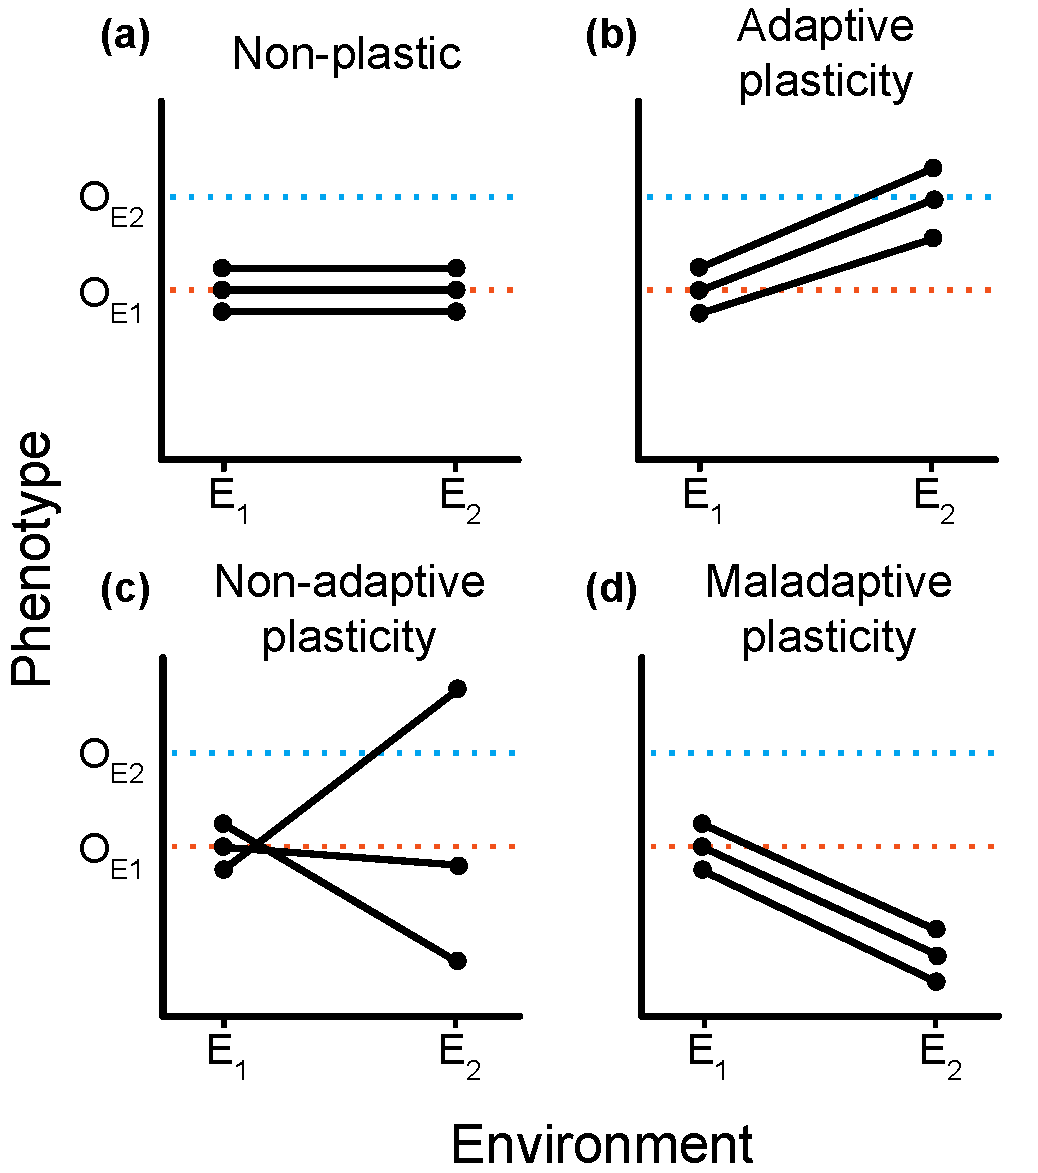
\includegraphics[width=\textwidth]{media/reaction-norms.pdf}
    \caption{\small
    \textbf{todo.}
    todo.
    }
    \label{fig:reaction-norms}
\end{figure}

% Feedback
%  - Ideas: color background red/blue
%  - Titles on (a), (b), (c), (d)?
%    - Swap (c) & (d)
%    - non-plastic, adaptive plasticity, non-adaptive plasticity, maladaptive plasticity
%  - (e) environmental scenario/environment
% - Increase font sizes
% - pull word that says time outside the arrow, make arrow smaller, make environment bar bigger => increase font size

% -- Plasticity as a source of cryptic variation --
Phenotypic plasticity allows for the accumulation of genetic variation in genomic regions that are unexpressed under current environmental conditions.
Such cryptic (``hidden'') genetic variation can serve as a source of diversity in the population, upon which selection can act when the environment changes \citep{schlichting_hidden_2008,levis_evaluating_2016}.  
It remains unclear to what extent and under what circumstances this cryptic variation caches adaptive potential or merely accumulates deleterious alleles \citep{gibson_uncovering_2004,paaby_cryptic_2014,zheng_cryptic_2019}.

% -- Genes as followers --
The ``genes as followers'' hypothesis (also known as the ``plasticity first'' hypothesis) predicts that phenotypic plasticity may facilitate adaptive evolutionary change by producing variants with enhanced fitness under stressful or novel conditions \citep{west-eberhard_developmental_2003,schwander_genes_2011,levis_evaluating_2016}. 
Environmentally-induced trait changes can be refined through selection over time (\textit{i.e.}, genetic accommodation).
Further, selection may drive plastic phenotypes to lose their environmental dependence over time in a process known as genetic assimilation \citep{west-eberhard_developmental_2005,pigliucci_phenotypic_2006,crispo_baldwin_2007,schlichting_phenotypic_2014,levis_evaluating_2016}. 
In this way, environmentally-induced phenotypic changes can precede an evolutionary response.

% -- Plastic rescue + wrap up on plasticity background? --
Phenotypic plasticity may also ``rescue'' populations from extinction under changing environmental conditions by buffering populations against novel stressors.
This buffer promotes stability and persistence and grants populations time to further adapt to rapidly changing environmental conditions \citep{west-eberhard_developmental_2003,chevin_when_2010}. 

Disparate predictions about how phenotypic plasticity may shift the course of subsequent evolution are not necessarily mutually exclusive.
Genetic and environmental contexts determine if, and to what extent, phenotypic plasticity promotes or constrains subsequent evolution.
Figure \ref{fig:reaction-norms} overviews how we might expect different forms of phenotypic plasticity to result in different evolutionary responses after an environmental change.

%%%%%%%%%%%%%%%%%%%%%%
% -- Digital evolution --
%%%%%%%%%%%%%%%%%%%%%%
Experimental studies investigating the relationship between phenotypic plasticity and evolutionary outcomes can be challenging to conduct in natural systems.
Such experiments would require the ability to irreversibly toggle plasticity followed by long periods of evolution during which detailed phenotypic data would need to be collected.
Digital evolution experiments have emerged as a powerful research framework from which evolution can be studied.
In digital evolution, self-replicating computer programs (digital organisms) compete for resources, mutate, and evolve following Darwinian dynamics  \citep{wilke_biology_2002}.
Digital evolution studies balance the speed and transparency of mathematical and computational simulations with the open-ended realism of laboratory experiments.
Modern computers allow us to observe many generations of digital evolution at tractable time scales; thousands of generations can take mere minutes as opposed to months, years, or millennia.
Digital evolution systems also allow for perfect, non-invasive data tracking.
Such transparency permits the tracking of complete evolutionary histories within an experiment, which circumvents the historical problem of drawing evolutionary inferences using incomplete records (from frozen samples or fossils) and extant genetic sequences.
Additionally, digital evolution systems allow for experimental manipulations and analyses that go beyond what is possible in wet-lab experiments.
Such analyses have included exhaustive knockouts of every site in a genome to identify the functionality of each \citep{lenski_evolutionary_2003},
comprehensive characterization of local mutational landscapes \citep{lenski_genome_1999,canino-koning_fluctuating_2019},
and the real-time reversion of all deleterious mutations as they occur to isolate their long-term effects on evolutionary outcomes \citep{covert_experiments_2013}. 
Furthermore, digital evolution studies allow us to directly toggle the possibility for adaptive plastic responses to evolve, which enables us to empirically test hypotheses that were previously relegated to theoretical analyses.

%%%%%%%%%%%%%%%%%%%%%%
% -- Overview of what we're testing / doing --
%%%%%%%%%%%%%%%%%%%%%%
In this work, we use the Avida Digital Evolution Platform \citep{ofria_avida:_2009}.
Avida is an open-source system that has been used to conduct a wide range of well-regarded studies on evolutionary dynamics, including 
the origins of complex features \citep{lenski_evolutionary_2003},
the survival of the flattest effect \citep{wilke_evolution_2001},
and the origins of reproductive division of labor \citep{goldsby_evolutionary_2014}.
% @AML: next bit is a little awkward
Our experiments build directly on previous studies in Avida that characterized the \textit{de novo} evolution of adaptive phenotypic plasticity \citep{clune_investigating_2007,lalejini_evolutionary_2016} as well as previous work investigating the evolutionary consequences of fluctuating environments for populations of non-plastic digital organisms \citep{li_digital_2004,canino-koning_fluctuating_2019}.
Of particular relevance, \cite{clune_investigating_2007} and \cite{lalejini_evolutionary_2016} experimentally demonstrated that adaptive phenotypic plasticity can evolve given the following four conditions (as identified by \citealt{ghalambor_behavior_2010}):
(1) populations experience temporal environmental variation,
(2) these environments are differentiable by reliable cues,
(3) each environment favors different phenotypic traits,
and (4) no single phenotype exhibits high fitness across all environments.
We build on this previous work, but we shift our focus from the evolutionary causes of adaptive phenotypic plasticity to investigate its evolutionary consequences in a fluctuating environment.

%%%%%%%%%%%%%%%%%

% - what we did -
Each of our experiments are divided into two phases: in phase one, we precondition sets of founder organisms with differing plastic or non-plastic adaptations;
in phase two, we examine the subsequent evolution of populations founded with organisms from phase one under specific environmental conditions (Figure \ref{fig:experimental-design}).
First, we examine the evolutionary histories of phase two populations to test whether adaptive plasticity constrained subsequent genomic and phenotypic changes. 
Next, we evaluate how adaptive plasticity influences how well populations produced by each type of founder can evolve and retain novel adaptive traits.
Finally, we examine lineages to determine whether adaptive plasticity facilitated the accumulation of cryptic genetic variation that would prove deleterious when the environment changed. 

%%%%%%%%%%%%%%%%%%%%%%
% - Overview of findings -
%%%%%%%%%%%%%%%%%%%%%%
We found that the evolution of adaptive plasticity reduced subsequent rates of evolutionary change in a cyclic environment.
The non-plastic populations underwent more frequent selective sweeps and accumulated many more genetic changes over time, as non-plastic populations relied on genetic variation from \textit{de novo} mutations to continuously readapt to environmental changes. 
The evolution of adaptive phenotypic plasticity buffered populations against environmental fluctuations, whereas repeated selective sweeps in non-plastic populations drove the accumulation of deleterious mutations and the loss of secondary beneficial traits via deleterious hitchhiking.
As such, adaptively plastic populations were better able to retain novel traits than their non-plastic counterparts.
In general, the evolution of adaptive phenotypic plasticity shifted evolutionary dynamics to be more similar to that of populations evolving in a static environment than to non-plastic populations evolving in an identical fluctuating environment. 

% We additionally found no evidence of delthat the evolution of adaptive phenotypic plasticity 
% In addition, we did not find evidence that the evolution of adaptive plasticity resulted in increased rates of deleterious mutation accumulation. 


%%%%%%%%%%%%%%%%%%%%%%%%%%%%%%%%%%%%%%%%%%%%%%%%%%%%%%%%%%%%%%%
% JOURNAL INSTRUCTIONS
% This section may be divided by subheadings and should contain sufficient detail so that when read in conjunction with cited references, all procedures can be repeated. For experiments reporting results on animal or human subject research, an ethics approval statement should be included in this section (for further information, see the Bioethics section.)
%%%%%%%%%%%%%%%%%%%%%%%%%%%%%%%%%%%%%%%%%%%%%%%%%%%%%%%%%%%%%%%

\section{Materials and Methods}

\subsection{The Avida Digital Evolution Platform}

% -- Define digital organisms --
Avida is a study system wherein self-replicating computer programs (digital organisms) compete for space on a finite toroidal grid \citep{ofria_avida:_2009}.
Each digital organism is defined by a linear sequence of program instructions (its genome) and a set of virtual hardware components used to interpret and express those instructions.
Genomes are expressed sequentially except when the execution of one instruction (\textit{e.g.}, a ``jump'' instruction) deterministically changes which instruction should be executed next.
Genomes are built using an instruction set that is both robust (\textit{i.e.}, any ordering of instructions is syntactically valid, though not necessarily meaningful) and Turing Complete (\textit{i.e.}, able to represent any computable function, though not necessarily in an efficient manner).
The instruction set includes operations for basic computations, flow control (\textit{e.g.}, conditional logic and looping), input, output, and self-replication.
% The virtual hardware set includes components such as a central processing unit (CPU) for executing instructions, registers to store values, buffers for inputs and outputs, and memory stacks \citep{ofria_avida:_2009}.

% -- Define reproduction & mutation --
Organisms in Avida reproduce asexually by copying their genome instruction-by-instruction and then dividing.
However, copy operations are imperfect and can result in single-instruction substitution mutations in an offspring's genome.
For this work, we configured copy operations to err at a rate of one expected mutation for every 400 instructions copied (\textit{i.e.}, a per-instruction error rate of 0.0025).
We held individual genomes at a fixed length of 100 instructions; that is, we did not include insertion and deletion mutations.
We used fixed-length genomes to control for treatment-specific conditions resulting in the evolution of substantially different genome sizes \citep{supplemental_material}\footnote{
We repeated our experiments without genome size restrictions and observed qualitatively similar results (see supplemental material, \citealt{supplemental_material}).
}, which could, on its own, drive differences in evolutionary outcomes among experimental treatments.
When an organism divides in Avida, its offspring is placed in a random location on the toroidal grid, replacing any previous occupant.
For this work, we used the default 60 by 60 grid size, which limits the maximum population size to 3600 organisms.
As such, improvements to the speed of self-replication are advantageous in the competition for space.

% -- Define fitness/metabolic rate/improving replication speed --
During evolution, organism replication rates improve in two ways: by improving genome efficiency (\textit{e.g.}, using a more compact encoding) or by accelerating the rate at which the genome is expressed (their ``metabolic rate'').
An organism's metabolic rate determines the speed at which it executes instructions in its genome.
Initially, an organism's metabolic rate is proportional to the length of its genome, but that rate is adjusted as it completes designated tasks, such as performing Boolean logic computations \citep{ofria_avida:_2009}.
In this way, we can reward or punish particular phenotypic traits.

% \vspace{0.25cm}
\subsubsection{Phenotypic plasticity in Avida}

% -- Phenotypes & Phenotypic plasticity --
%   - What is a phenotype in Avida?
In this work, we measure a digital organism's phenotype as the set of Boolean logic functions that it performs in a given environment.
Sensory instructions in the Avida instruction set allow organisms to detect how performing a particular logic function would affect their metabolic rate (see supplemental material for more details, \citealt{supplemental_material}).
We define a phenotypically plastic organism as one that uses sensory information to alter which logic functions it performs based on the environment.

% -- Adaptive plasticity & non-adaptive plasticity --
Phenotypic plasticity in Avida can be adaptive or non-adaptive for a given set of environments.
Adaptive plasticity shifts net task expression closer to the optimum for the given environments.
Non-adaptive plasticity changes task expression in either a neutral or deleterious way.
In this work, optimal plasticity toggles tasks to always perfectly match the set of rewarded tasks for the given set of environments.

% \vspace{0.7cm}
\subsection{Experimental design}
\label{sec:methods:experiment}

\begin{figure}[h!]
    \centering
    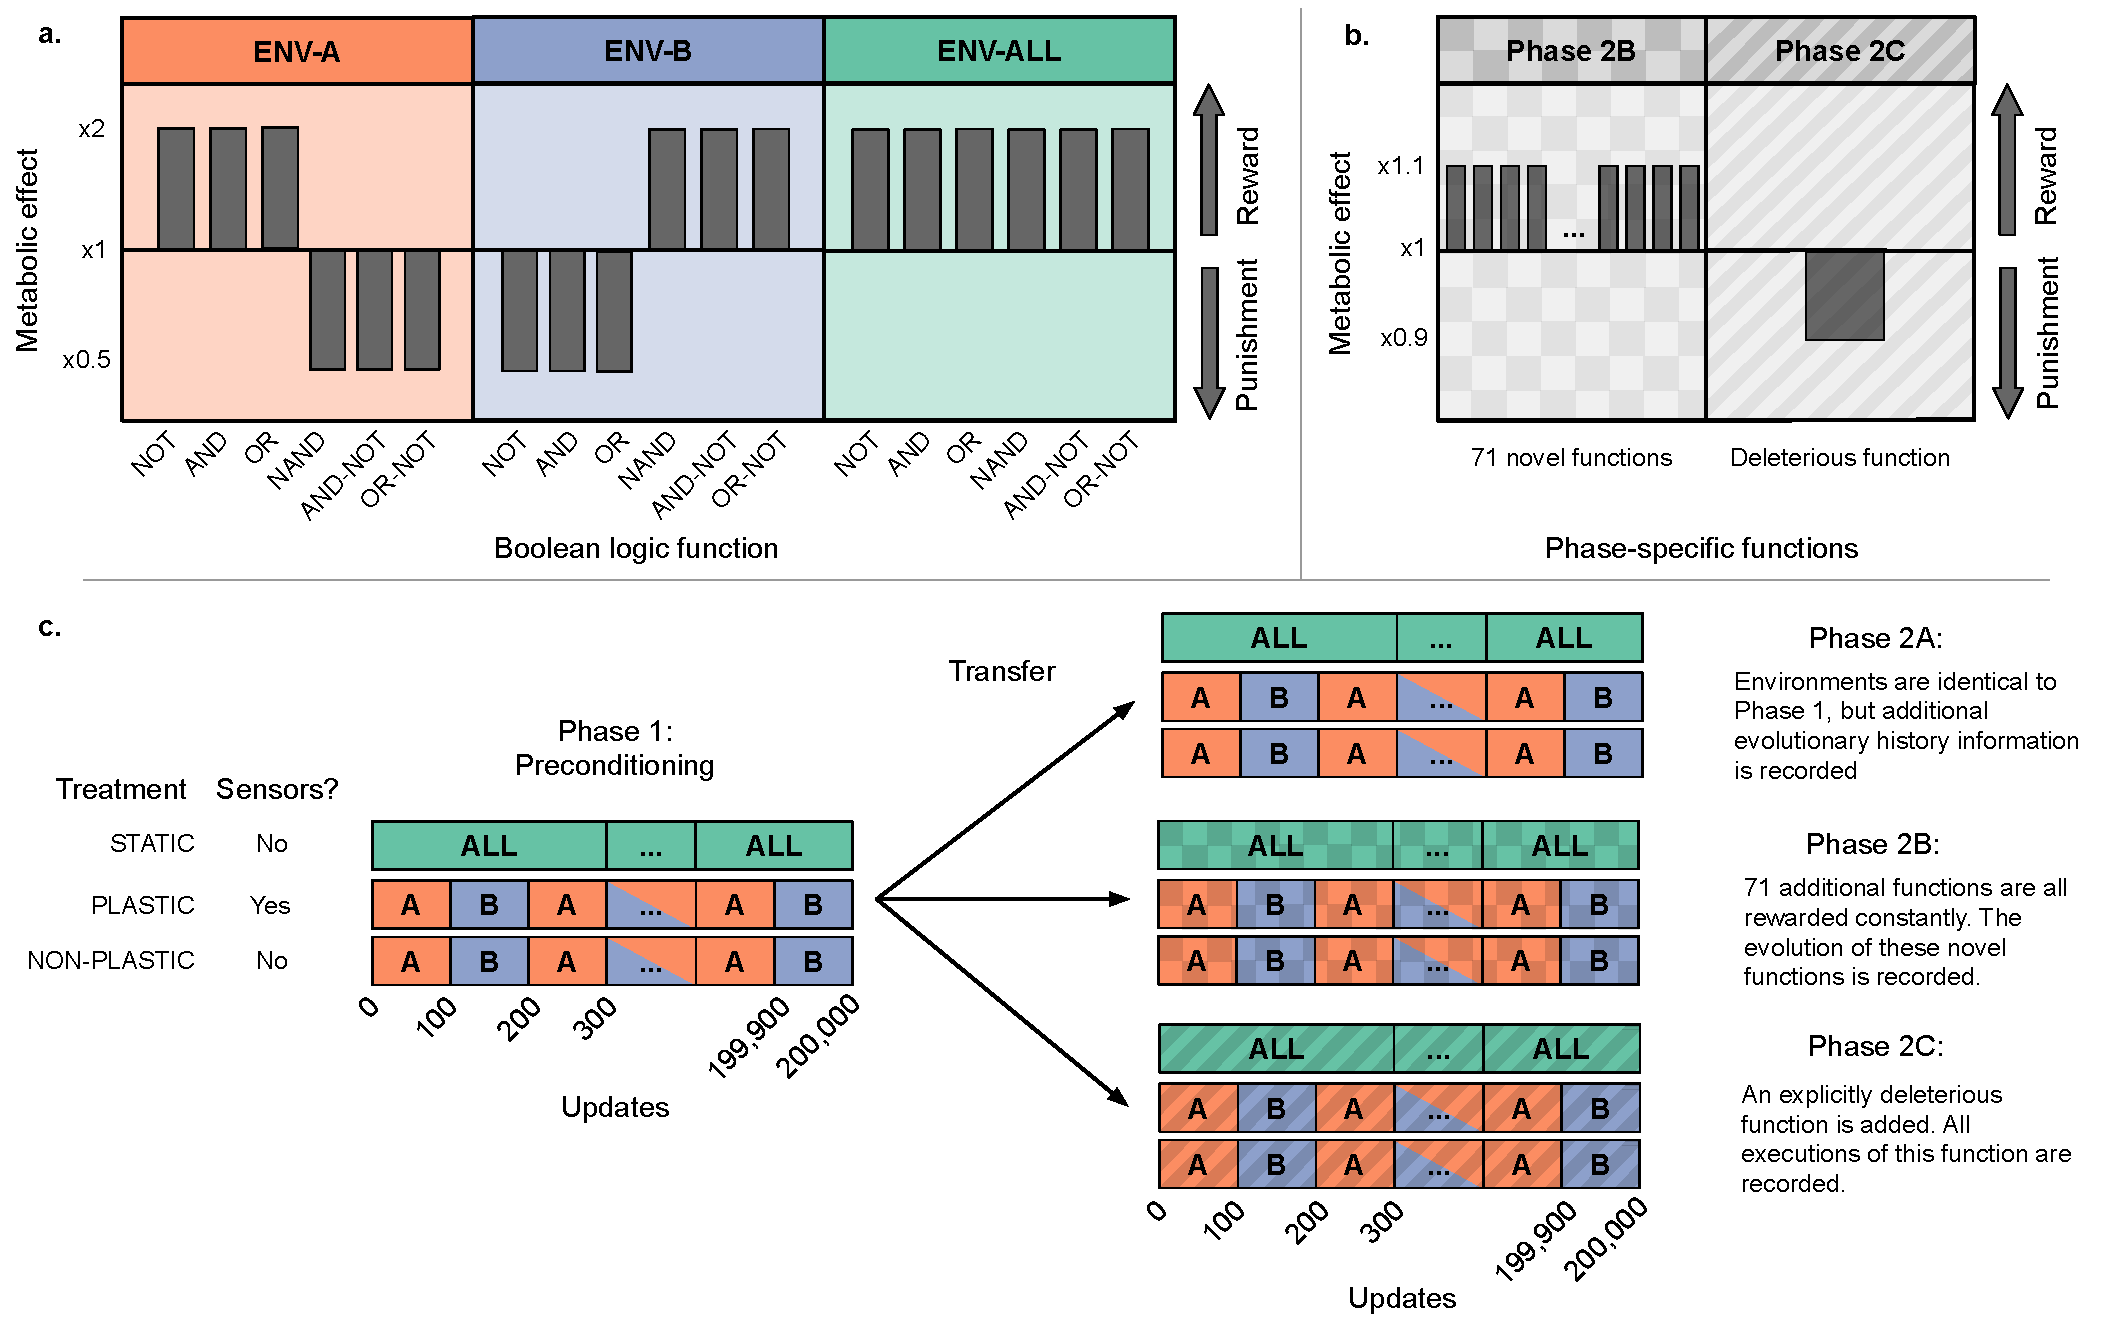
\includegraphics[width=1\textwidth]{media-experimental-design.pdf}
    \caption{\small
    \textbf{Overview of experimental design.}
    The first three plots in panel (a) show the environments used in every experiment and whether they reward or punish each base task.
    Additionally, the last two subplots in (a) show the additional tasks added in phases 2B and 2C.
    All novel tasks in phase 2B confer a 10\% metabolic reward, while executing the poisonous task in phase 2C causes a 10\% metabolic punishment (bars not drawn to scale).
    Panel (b) shows treatment differences and experimental phases.
    Treatments are listed on the left, with each treatment specifying its environmental configuration and whether sensors are functional.
    % consisting of an environment timeline and whether sensors are functional.
    % This also shows Phase 1, the preconditioning phase.
    We conducted three independent two-phase experiments, each described on the right.
    % We conducted experiments using three different second phases, as shown on the right.
    Phases 2B and 2C are textured to match their task definitions in panel (a).
    Phase one is repeated for \textit{each} experiment with 100 replicate populations per treatment per experiment.
    For each replicate at the end of phase one, we used an organism of the most abundant genotype to found the second phase population.
    All STATIC and NON-PLASTIC populations move on to phase two, but PLASTIC populations only continue to the second phase if their most abundant genotype exhibits optimal plasticity.
    Metrics are recorded only in phase two.
    }
    \label{fig:experimental-design}
\end{figure}

%%%%%%%%%%%%%%%%%%%%%%%%%%%%%%%%%%%%%%%%%%%%%%%%%
% OUTLINE
%%%%%%%%%%%%%%%%%%%%%%%%%%%%%%%%%%%%%%%%%%%%%%%%%
% Overview of experimental design - with diagram (not a subsubsection?)
% - Focused around diagram
% Environment implementations
% Specifications for Phase 1
% specifications for Phase 2A
% specifications for Phase 2B
% specifications for Phase 2C
%%%%%%%%%%%%%%%%%%%%%%%%%%%%%%%%%%%%%%%%%%%%%%%%%

% -- Treatments --
We conducted three independent experiments using Avida to investigate how the evolution of adaptive plasticity influences evolutionary outcomes in fluctuating environments.
For each experiment, we compared the evolutionary outcomes of populations evolved under three treatments (Figure \ref{fig:experimental-design}):
(1) a \textbf{PLASTIC} treatment where the environment fluctuates, and digital organisms can use sensory instructions to differentiate between environmental states;
(2) a \textbf{NON-PLASTIC} treatment with identical environment fluctuations, but where sensory instructions are disabled;
and (3) a \textbf{STATIC} control where organisms evolve in a constant environment.

% -- Experiment phases --
Each experiment was divided into two phases that each lasted for 200,000 updates\footnote{
    One update in Avida is the amount of time required for the average organism to execute 30 instructions.
    See \citep{ofria_avida:_2009} for more details.
} of evolution (Figure \ref{fig:experimental-design}), which is equivalent to approximately 30,000 to 40,000 generations.
In phase one of each experiment, we preconditioned populations to their treatment-specific conditions.
In phase two, we founded new populations with the evolved organisms from phase one and examined their subsequent evolution under given combinations of treatment and experimental conditions.
During phase two, we tracked and saved each population's evolutionary history as well as saving the full final population.
Phase one was for preconditioning only; all comparisons between treatments were performed on phase two data.

\subsubsection{Environments}
\label{sec:methods:experiment:environments}

% ----- ENVIRONMENTS -----
% traits_set_a <- c("not", "and", "or")
% traits_set_b <- c("nand", "ornot", "andnot")

% -- Environment definitions --
We constructed three experimental environments, abbreviated hereafter as ``ENV-A'', ``ENV-B'', and ``ENV-ALL''.
Figure \ref{fig:experimental-design} describes these environments based on whether each of six Boolean logic tasks (NOT, NAND, AND, OR-NOT, OR, and AND-NOT) is rewarded or punished.
A rewarded task performed by an organism doubles their metabolic rate, allowing them to execute twice as many instructions in the same amount of time.
A punished task halves an organism's metabolic rate.

% -- Treatment-specific environment details --
In both the PLASTIC and NON-PLASTIC treatments, the environment cycles between equal-length periods of ENV-A and ENV-B.
Each of these periods persist for 100 updates (approximately 15 to 20 generations).
Thus, populations experience a total of 1,000 full periods of ENV-A interlaced with 1,000 full periods of ENV-B during each experimental phase.

% -- Sensory instructions + control flow and controlling the capacity for plasticity --
Organisms in the PLASTIC treatments differentiate between ENV-A and ENV-B by executing one of six sensory instructions, each associated with a particular logical task; these sensory instructions detect whether their associated task is currently rewarded or punished.
By using sensory information in combination with execution flow-control instructions, organisms can conditionally perform different logic tasks depending on the current environmental conditions.

% \vspace{5mm}
\subsubsection{Experiment Phase 1 -- Environment preconditioning}
\label{sec:methods:experiment:phase-one}

For each treatment, we founded 100 independent populations from a common ancestral strain capable only of self-replication.
At the end of phase one, we identified the most abundant (\textit{i.e.}, dominant) genotype and sampled an organism with that genotype from each replicate population to found a new population for phase two.

For the PLASTIC treatment, we measure plasticity by independently testing a given genotype in each of ENV-A and ENV-B.
We discard phase one populations if the dominant genotype does not exhibit optimal plasticity.
This approach ensures that measurements taken on PLASTIC-treatment populations during the second phase of each experiment reflect the evolutionary consequences of adaptive plasticity.

% \vspace{5mm}
\subsubsection{Experiment Phase 2A -- Evolutionary change rate}
\label{sec:methods:exp:evolutionary-change-rate}

Phase 2A continued exactly as phase one, except we tracked the rates of evolutionary change in each of the PLASTIC-, NON-PLASTIC-, and STATIC-treatment populations.
Specifically, we quantified evolutionary change rates using four metrics (each described in Table~\ref{tab:metrics-definitions}):
(1) coalescence event count,
(2) mutation count,
(3) phenotypic volatility,
and (4) mutational robustness.

% \vspace{3mm}
\subsubsection{Experiment Phase 2B -- Novel task evolution}
\label{sec:methods:exp:novel-task-evolution}

Phase 2B extended the conditions of phase one by adding 71 novel Boolean logic tasks, which were always rewarded in all treatments \citep{ofria_avida:_2009}.
The original six phase one tasks (NOT, NAND, AND, OR-NOT, OR, and AND-NOT; hereafter called ``base'' tasks) continued to be rewarded or punished according to the particular treatment conditions.
% @CAO: line below can be restored (and reworded) if readers need help with the intuition.
%As such, in fluctuating environments, the six base tasks continued to fluctuate, but the additional 71 tasks were always rewarded; in static environments, performing any of the 77 logic tasks was always beneficial.
An organism's metabolic rate was increased by \novelTraitsReward\ for each novel task that it performed (limited to one reward per task).
This reward provided a selective pressure to evolve these tasks, but their benefits did not overwhelm the 100\% metabolic rate increase conferred by rewarded base tasks.
As such, populations in the PLASTIC and NON-PLASTIC treatments could not easily escape environmental fluctuations by abandoning the fluctuating base tasks.

During this experiment, we tracked the extent to which populations evolving under each treatment were capable of acquiring and retaining novel tasks.
Specifically, we used three metrics (each described in Table~\ref{tab:metrics-definitions}):
(1) final novel task count,
(2) novel task discovery,
and (3) novel task loss.

% \vspace{5mm}
\subsubsection{Experiment Phase 2C -- Deleterious instruction accumulation}
\label{sec:methods:exp:deleterious-instruction-accumulation}

Phase 2C extended the instruction set of phase one with a \code{poison} instruction.
When an organism executes a \code{poison} instruction, it performs a ``poisonous'' task, which reduces the organism's metabolic rate (and thus reproductive success) but does not otherwise alter the organism's function.
We imposed a 10\% penalty each time an organism performed the poisonous task, making the \code{poison} instruction explicitly deleterious to execute.
We did not limit the number of times that an organism could perform the poisonous task, and as such, organisms could perform the poisonous task as many times as they executed the \code{poison} instruction.

We tracked the number of times each organism along the dominant lineage performed the poisonous task.
Specifically, we used two metrics (each described in Table~\ref{tab:metrics-definitions}):
(1) final poisonous task count and (2) poisonous task acquisition count.

% \vspace{5mm}
\subsection{Experimental analyses}

% Evolutionary history

% Lineages and phylogenies
% - number of coalescence
% - mutation accumulation
% - phenotypic volatility
% - mutational stability
% - novel task performance
% - novel task discovery
% - genetic architectures


%%%%%%%%% BOX %%%%%%%%%%%%
% this is my current "definition" environment
% \newtcolorbox[auto counter]{definitions}[1][] {
%   enhanced,
%   breakable,
%   arc=0mm,
%   title={\textbf{Box \thetcbcounter. Metrics}},
%   #1
% }

% \begin{definitions}[colback=blue!5!white,colframe=blue!75!black,label=box:metrics]

% Hello world.

% \end{definitions}
%%%%%%%%%%%%%%%%%%%%%%%%%%

% @AML: Not sure the best way to start the description of each metric. 

\newcommand{\SweepsMetricName}{
Coalescence event count
}
\newcommand{\SweepsMetricDesc}{
Number of coalescence events that have occurred, which indicates the frequency of selective sweeps in the population.
}

\newcommand{\MutationCountMetricName}{
Mutation count
}
\newcommand{\MutationCountMetricDesc}{
Sum of all mutations that have occurred along a lineage.
}

% Phenotypic volatility => 
% - 
\newcommand{\PhenotypicVolatilityMetricName}{
Phenotypic volatility
}
\newcommand{\PhenotypicVolatilityMetricDesc}{
Number of instances where parent and offspring phenotypic profiles do not match along a lineage.
% Phenotypic volatility as defined here indicates the rate at which accumulated genetic changes actually change the phenotype along a lineage.
}

\newcommand{\MutationalStabilityMetricName}{
Mutational robustness
% OLD: Mutational stability
}
\newcommand{\MutationalStabilityMetricDesc}{
Proportion of mutations (from the set of all possible one-step mutations) that do not change the phenotypic profile of a focal genotype. We also measured \textit{realized mutational robustness}, which is the proportion of mutated offspring along a lineage whose phenotypic profile matches that of their parent. 
% OLD DEFS:
% - Proportion of mutated offspring along a lineage whose phenotypic profile matches that of their parent. 
% - Proportion of mutants whose phenotypic profile matches that of their parent. Two variations were recorded: lineage mutational stability which examines the mutated offspring along a lineage, and neighborhood mutational stability which examines a set of possible mutations on a given genotype.
}


% Mutational stability => phenotypic stability / mutational robustness
% - Lineage => realized phenotypic stability / realized stability / realized mutational robustness
% - Neighborhood => potential phenotypic stability / potential stability / potential mutational robustness

% - Mutational robustness
% - Realized mutational robustness

\newcommand{\TaskPerformanceMetricName}{
Final novel task count
}
\newcommand{\TaskPerformanceMetricDesc}{
Count of unique novel tasks performed by the representative organism in a final population from experiment \hyperref[sec:methods:exp:novel-task-evolution]{phase 2B}. 
This metric can range from 0 to 71 and measures how well the fitness landscape was exploited  at a given point in time.
% (\textit{i.e.}, the mapping between genetic space and phenotype space)
% We focused on an organism from the dominant genotype at the end of the experiment as the most representative phenotype in the evolved population.
% Final task count is equivalent to the ``task performance'' metric in \citep{canino-koning_fluctuating_2019}.
}

\newcommand{\TaskDiscoveryMetricName}{
Novel task discovery
}
\newcommand{\TaskDiscoveryMetricDesc}{
Number of unique novel tasks ever performed along a given lineage in experimental \hyperref[sec:methods:exp:novel-task-evolution]{phase 2B}, even if a task is later lost.
This metric can range from 0 to 71 and measures a given lineage's level of exploration of the fitness landscape.
}

\newcommand{\TaskLossMetricName}{
Novel task loss
}
\newcommand{\TaskLossMetricDesc}{
Number of instances along a given lineage from experimental \hyperref[sec:methods:exp:novel-task-evolution]{phase 2B} where a novel task is performed by a parent but not its offspring. 
This metric measures how often a given lineage fails to retain evolved traits over time.
}

\newcommand{\FinalPoisonMetricName}{
Final poisonous task count
}
\newcommand{\FinalPoisonMetricDesc}{
Number of times the poisonous task is performed by the representative organism from a final population from experiment \hyperref[sec:methods:exp:deleterious-instruction-accumulation]{phase 2C}.
}

\newcommand{\LineagePoisonMetricName}{
Poisonous task acquisition count
}
\newcommand{\LineagePoisonMetricDesc}{
Number of instances along a given lineage where a mutation causes an offspring to perform the poisonous task more times than its parent. 
}

\newcommand{\ArchitectureVolatilityMetricName}{
Architectural volatility
}
\newcommand{\ArchitectureVolatilityMetricDesc}{
The average number of loci in the genome that change function per mutation along a lineage. 
% @AML: The average number of mutations that cause a change in function along a lineage. 
%Loci function is denoted as the combination of task machinery, plasticity machinery, vestigial machinery for both ENV-A and ENV-B tasks, as well as replication and required machinery. 
}

\newcommand*{\thead}[1]{\multicolumn{1}{c}{\bfseries #1}}

\setlength{\tabcolsep}{16pt}
\renewcommand{\arraystretch}{1.5}
\begin{table}[ht]
    \centering
    
    \rowcolors{2}{gray!25}{white}
    \begin{tabularx}{\linewidth}{lX} % p{10cm}
        \rowcolor{gray!50}
        \hline 
        \thead{Metric} & \thead{Description}   \\
        \hline
        \SweepsMetricName & \SweepsMetricDesc \\
        \MutationCountMetricName & \MutationCountMetricDesc \\
        \PhenotypicVolatilityMetricName & \PhenotypicVolatilityMetricDesc \\
        % \GenotypicFidelityMetricName &         \GenotypicFidelityMetricDesc \\
        % \PhenotypicFidelityMetricName &         \PhenotypicFidelityMetricDesc \\
        \MutationalStabilityMetricName & \MutationalStabilityMetricDesc \\
        % (architecture metric(s)) & \\
        %\ArchitectureVolatilityMetricName & \ArchitectureVolatilityMetricDesc \\
        \TaskPerformanceMetricName & \TaskPerformanceMetricDesc \\
        \TaskDiscoveryMetricName & \TaskDiscoveryMetricDesc \\
        \TaskLossMetricName & \TaskLossMetricDesc \\
        \FinalPoisonMetricName & \FinalPoisonMetricDesc \\
        \LineagePoisonMetricName & \LineagePoisonMetricDesc \\
        \hline
    \end{tabularx}
    
    \caption{\textbf{Metric descriptions.}}
    \label{tab:metrics-definitions}
\end{table}




% naive environment = what organism experiencing
% alternative environment = what organism is not currently experiencing

% - How we extracted representative lineages -
For each of our experiments, we tracked and analyzed the phylogenetic histories of evolving populations during phase two.
For each replicate, we identified an organism with the most abundant genotype in the final evolved population, and we used it as a \textit{representative organism} for further analysis.
% We then isolated the lineage from the founding organism to the representative organism, which we used as the representative lineage for further analysis.
We used the lineage from the founding organism to the representative organism as the \textit{representative lineage} for further analysis.
We manually inspected evolved phylogenies and found no evidence that any of our experimental treatments supported long-term coexistence.
As such, each of the representative lineages reflect the majority of evolutionary history from a given population at the end of our experiment.

% -- PHENOTYPIC PROFILE --
% DEFINE PHENOTYPIC PROFILE - metric definitions will use this.
Some of our metrics (Table \ref{tab:metrics-definitions}) required us to measure genotype-by-environment interactions.
Importantly, in the fluctuating environments, we needed to differentiate phenotypic changes that were caused by mutations from those that were caused by environmental changes.
To accomplish this, we produced organisms with the given focal genotype, measured their phenotype in each environment, and aggregated the resulting phenotypes to create a \textit{phenotypic profile}.
Although organisms with different genotypes may express the same set of tasks across environments, their phenotypic profiles may not necessarily be the same.
For example, an organism that expresses NOT in ENV-A and NAND in ENV-B has a distinct phenotypic profile from one that expresses NAND in ENV-A and NOT in ENV-B.

% -- GENETIC MANIPULATION / MUTATIONAL NEIGHBORHOOD --
% How do we produce mutants for analyses?
While most analyses employed here are retrospective metrics applied to lineages, digital evolution allows precise manipulations on individual organisms and genomes.
Mutational robustness uses this technique when looking at the possible mutations on a representative genotype.
Genomes in Avida are linear sequences of instructions, and as such possible mutations can be simulated by substituting other instructions at the desired site.
Indeed, the mutational robustness of a genotype examines all one-step mutations (\textit{i.e.}, each mutation where exactly one instruction is substituted).
This allows us the disentangle whether results of the lineage metrics are a consequence of evolved genetic architectures or otherwise.
%purely the results of selection.


\subsection{Statistical analyses}

Across all of our experiments, we differentiated between sample distributions using non-parametric statistical tests.
For each major analysis, we first performed a Kruskal-Wallis test \citep{kruskal_use_1952} to
determine if there were significant differences in results from the PLASTIC, NON-PLASTIC, and STATIC treatments (significance level $\alpha=0.05$).
If so, we applied a Wilcoxon rank-sum test \citep{kotz_individual_1992} to distinguish between pairs of treatments.
We applied Bonferroni corrections for multiple comparisons \citep{rice_analyzing_1989} where appropriate.

\subsection{Software availability}

We conducted our experiments using a modified version of the Avida software, which is open source and freely available on \href{https://github.com/amlalejini/evolutionary-consequences-of-plasticity}{GitHub} \citep{supplemental_material}.
We used Python for data processing, and we conducted all statistical analyses using R version 4 \citep{r_core_team_r_v4}.
We used the tidyverse collection of R packages \citep{r_tidyverse_2019} to wrangle data, and we used the following R packages for analysis, graphing, and visualization:
ggplot2 \citep{R-ggplot2},
cowplot \citep{R-cowplot},
Color Brewer \citep{harrower_colorbrewerorg_2003,R-Brewer_2014},
rstatix \citep{R-rstatix},
ggsignif \citep{R-ggsignif},
scales \citep{R-scales},
Hmisc \citep{R-Hmisc},
fmsb \citep{R-fmsb},
and boot \citep{R-boot}.
We used R markdown \citep{rmarkdown} and bookdown \citep{R-bookdown} to generate web-enabled supplemental material.
All of the source code for our experiments and analyses, including configuration files and guides for replication, can be found in our supplemental material, which is hosted on \href{https://github.com/amlalejini/evolutionary-consequences-of-plasticity}{GitHub} \citep{supplemental_material}.
Additionally, our experimental data is available on the Open Science Framework at \url{https://osf.io/sav2c/} \citep{osf_data}.

%%%%%%%%%%%%%%%%%%%%%%%%%%%%%%%%%%%%%%%%%%%%%%%%%%%%%%%%%%%%
% INSTRUCTIONS:
% This section may be divided by subheadings. Footnotes should not be used and must be transferred to the main text.
%%%%%%%%%%%%%%%%%%%%%%%%%%%%%%%%%%%%%%%%%%%%%%%%%%%%%%%%%%%%

\section{Results}

\subsection{Adaptive phenotypic plasticity slows evolutionary change in fluctuating environments}


\begin{figure}[h!]
    \centering
    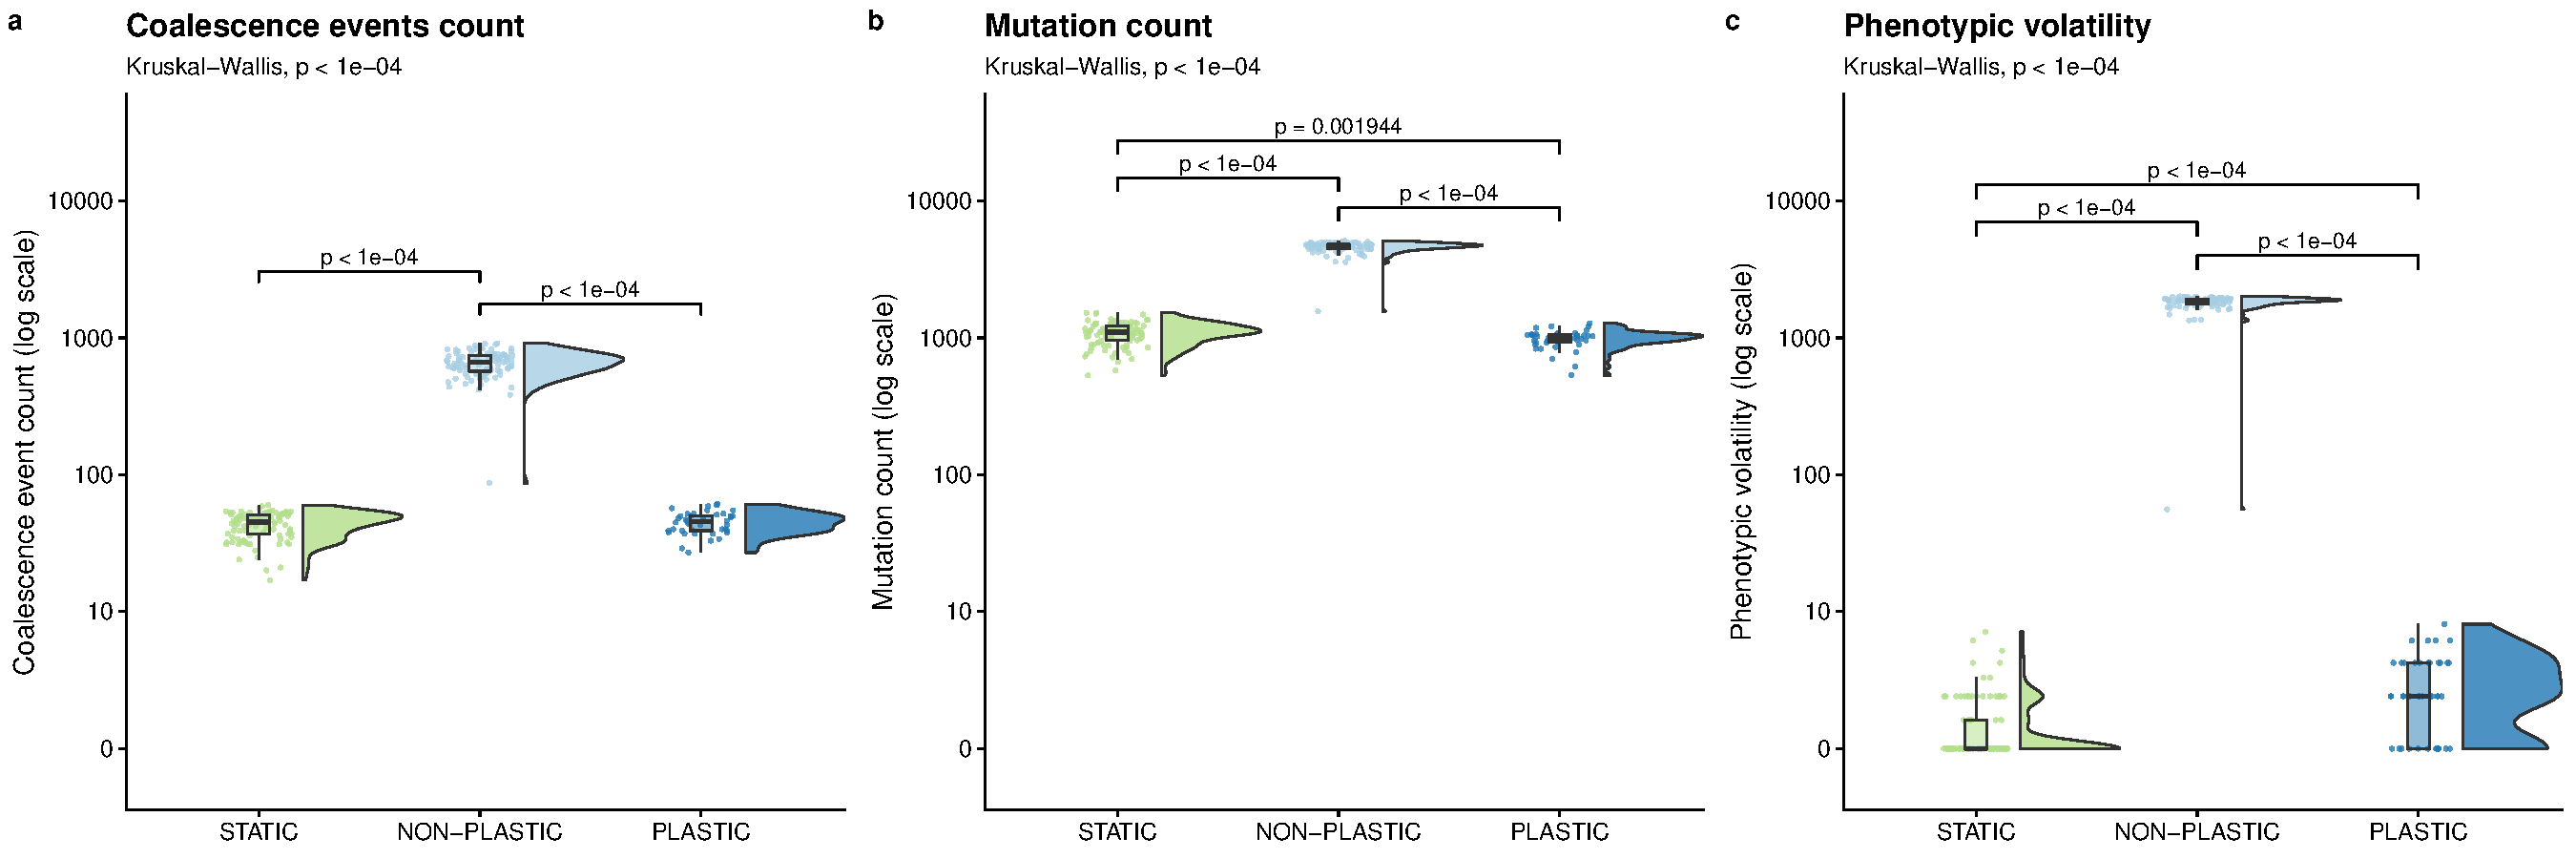
\includegraphics[width=1\textwidth]{media-evolutionary-change-magnitude-panel.pdf}
    \caption{\small
    \textbf{Magnitude of evolutionary change.}
    Raincloud plots \citep{allen_raincloud_2019} of
    (a) coalescence event count,
    (b) mutation count,
    and (c) phenotypic volatility.
    See Table \ref{tab:metrics-definitions} for descriptions of each metric.
    Each plot is annotated with statistically significant comparisons (Bonferroni-corrected pairwise Wilcoxon rank-sum tests).
    Note that adaptive phenotypic plasticity evolved in \evolutionaryChangeRatePlasticReps\ of \evolutionaryChangeRateReplicates\ replicates from the PLASTIC treatment during phase one of this experiment; we used this more limited group to found \evolutionaryChangeRatePlasticReps\ phase-two PLASTIC replicates from which we report these PLASTIC data.
    }
    \label{fig:evolutionary-dynamics-magnitude}
\end{figure}


%%%%%%%%%%%%%%%%%%%%%%%%%%%%%%%%%
% Results to report (2021-02-08 experiment)
% ----- GENERATIONS -----
% - average generations elapsed (of a population)
%   - NON-PLASTIC (median: 41768.65) > PLASTIC (median: 31697.65) > STATIC (median: 30839.75)
%   condition     mean    sd
%   <chr>        <dbl> <dbl>
% 1 NON-PLASTIC 41090. 2702.
% 2 PLASTIC     31016. 2615.
% 3 STATIC      30002. 3011.

%
% ----- SWEEPS -----
% - coalescence events (total)
%   - NON-PLASTIC (median: 663.5) > ( PLASTIC (median: 45.5) ~~ STATIC (median: 45) )
% - Average number of generations between coalescence events (gens / sweeps)
%   - ( PLASTIC (median: 685.001780758557) ~~ STATIC (median: 693.676265008576) ) > NON-PLASTIC (median: 62.0184902295191)
%
% ----- PHENOTYPIC VOLATILITY -----
% - phenotypic volatility (total)
%   - i.e., total number of times phenotypes change along lineages
%   - NON-PLASTIC (median: 1868) > PLASTIC (median: 2) > STATIC (median: 0)
% - phenotypic volatility / lineage length
%   - i.e., how often do genomic changes reflect changes in phenotype?
%   - NON-PLASTIC (median: 0.437) > PLASTIC (median: 0.0022) > STATIC (median: 0)
% - phenotypic volatility / generations
%   - i.e., per-offspring rate of phenotypic changes
%   - NON-PLASTIC (median: 0.0447) > PLASTIC (median: 6.33e-05) > STATIC (median: 0)
%
% ----- MUTATION ACCUMULATION -----
% - mutation accumulation (total)
%   - NON-PLASTIC (median: 4657.5) > STATIC (median: 1100) > PLASTIC (median: 998.5)
% - mutation accumulation / lineage length
%   - NON-PLASTIC (median: 1.10048311715591) > STATIC (median: 1.03794597464116) > PLASTIC (median: 1.0328599144651)
% - mutation accumulation / generation
%   - NON-PLASTIC (median: 0.11) > STATIC (median: 0.0368) > PLASTIC (median: 0.0319)
%
% ----- MUTATIONAL EFFECTS -----
% - fraction of mutational steps that alter (aggregate) phenotype
%   - NON-PLASTIC (mean: 0.434007, CI [0.4242,  0.4406]) > PLASTIC (mean: 0.002717008, 0.0020,  0.0035) > STATIC (mean: 0.0006788834, CI [0.0004,  0.0009])
% - fraction of phenotype-altering mutation steps that alter unexpressed phenotype (PLASTIC condition only)
%   - mean: 0.8247126 CI [0.7443,  0.8994]
% - fraction of mutations that affect unexpressed phenotype that are deleterious (PLASTIC only)
%   - mean: 0.5172414 CI [0.4402,  0.5977]
% - fraction of mutations that affect unexpressed phenotype that are beneficial (PLASTIC only)
%   - mean: 0.4827586 CI [0.4046,  0.5598]
%%%%%%%%%%%%%%%%%%%%%%%%%%%%%%%%%

% -- Magnitude of evolutionary change --
%  - Selective sweeps
%  - Mutation accumulation
%  - Phenotypic volatility
In experimental phase 2A,
we tested whether adaptive phenotypic plasticity constrained or promoted subsequent evolutionary change in a fluctuating environment.
First, we compared the total amount of evolutionary change in populations evolved under the PLASTIC, NON-PLASTIC, and STATIC treatments as measured by coalescence event count, mutation count, and phenotypic volatility (Figure \ref{fig:evolutionary-dynamics-magnitude}).
According to each of these metrics, NON-PLASTIC populations experienced a larger magnitude of evolutionary change than either PLASTIC or STATIC populations.
We observed significantly higher coalescence event counts in NON-PLASTIC populations than in PLASTIC or STATIC populations (Figure \ref{fig:evolutionary-dynamics-magnitude}\hyperref[fig:evolutionary-dynamics-magnitude]{a}).
NON-PLASTIC lineages had significantly higher mutation counts (Figure \ref{fig:evolutionary-dynamics-magnitude}b) and phenotypic volatility than PLASTIC or STATIC lineages (Figure \ref{fig:evolutionary-dynamics-magnitude}c).

% -- Elapsed generations --
Changing environments have been shown to increase generational turnover in Avida populations \citep{canino-koning_evolution_2016}, which could explain why we observe a larger magnitude of evolutionary change at the end of 200,000 updates of evolution in NON-PLASTIC populations.
Indeed, we found that significantly more generations of evolution elapsed in NON-PLASTIC populations (mean of $41090\pm2702$ std. dev.) than in PLASTIC (mean of $31016\pm2615$ std. dev.) or STATIC (mean of $30002\pm3011$ std. dev.) populations during phase 2A (corrected Wilcoxon rank-sum tests, p $<10^{-4}$).

% -- Rate of evolutionary change => intuition --
To evaluate whether increased generational turnover explains the greater magnitude of evolutionary change in NON-PLASTIC populations, we examined the average number of generations between coalescence events and the realized mutational robustness of lineages (Table \ref{tab:metrics-definitions}).
A coalescence event indicates a selective sweep, which is a hallmark of adaptive evolutionary change.
Realized mutational robustness measures the frequency that mutations cause phenotypic changes along a lineage.
We expect that static conditions should favor fit lineages with high realized mutational robustness that no longer undergo rapid adaptive change and hence do not trigger frequent coalescence events.
Under fluctuating conditions, however, lineages must be composed of plastic organisms if they are to maintain both high fitness and realized mutational robustness.
Without plasticity, we expect fluctuating conditions to produce lineages with low realized mutational robustness and frequent coalescence events as populations must continually acquire and fix mutations to readapt to the environment.


\begin{figure}[h!]
    \centering
    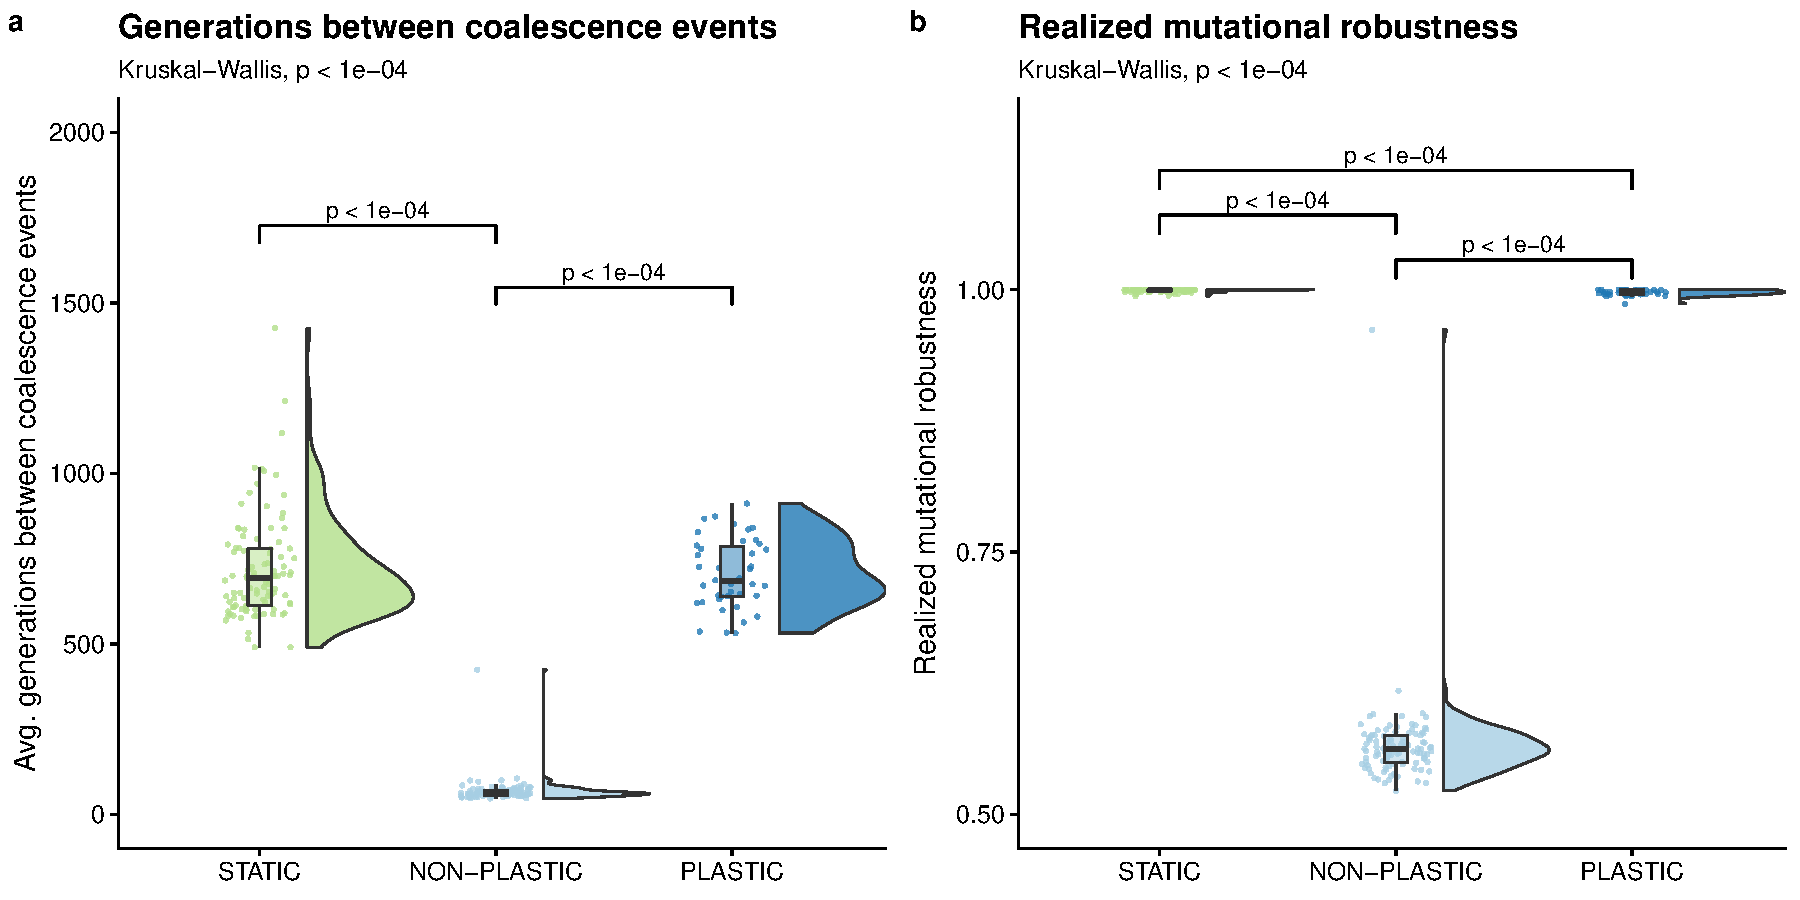
\includegraphics[width=0.66\textwidth]{media-evolutionary-change-pace-panel.pdf}
    \caption{\small
    \textbf{Pace of evolutionary change.}
    Raincloud plots of
    (a) average number of generations between coalescence events,
    and (b) realized mutational robustness (Table \ref{tab:metrics-definitions}).
    Each plot is annotated with statistically significant comparisons (Bonferroni-corrected pairwise Wilcoxon rank-sum tests).
    }
    \label{fig:evolutionary-dynamics-rate}
\end{figure}

% -- Rate of evolutionary change => findings --
On average, significantly fewer generations elapsed between coalescence events in NON-PLASTIC populations than in either PLASTIC or STATIC populations (Figure \ref{fig:evolutionary-dynamics-rate}a).
We also found that both STATIC and PLASTIC lineages exhibited higher realized mutational robustness relative to that of NON-PLASTIC lineages (Figure \ref{fig:evolutionary-dynamics-rate}b); that is, mutations observed along NON-PLASTIC lineages more often caused phenotypic changes in offspring.
Overall, our results indicate that NON-PLASTIC populations underwent more rapid (and thus a greater amount of) evolutionary change than either PLASTIC or STATIC populations.

% -- Mutational stability in static and plastic lineages --
While both STATIC and PLASTIC lineages exhibited high realized mutational robustness, we found that STATIC lineages exhibited higher realized robustness than PLASTIC lineages (Figure \ref{fig:evolutionary-dynamics-rate}b).
Overall, there were rare instances of mutations that caused a change in phenotypic profile across all PLASTIC lineages.
Of these mutations, we found that over 80\% (83 out of 102) of changes to phenotypic profiles were cryptic.
That is, the mutations affected traits that would not have been expressed in the environment that the organism was born into but would have been expressed had the environment changed.

\begin{figure}[ht!]
    \centering
    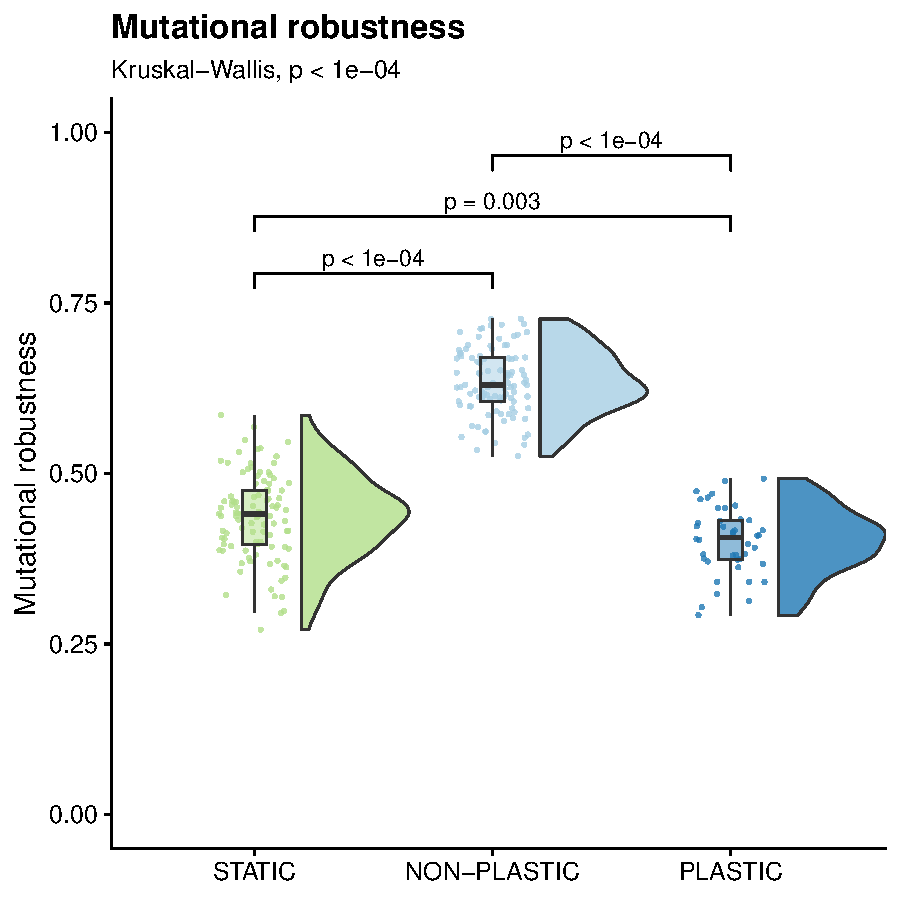
\includegraphics[width=0.33\textwidth]{media-mutational-robustness.pdf}
    \caption{\small
        \textbf{Mutational robustness.}
        Raincloud plot of mutational robustness of each representative genotype (Table \ref{tab:metrics-definitions}).
        The plot is annotated with statistically significant comparisons (Bonferroni-corrected pairwise Wilcoxon rank-sum tests).
    }
    \label{fig:mutational-robustness}
\end{figure}

% -- mutational landscaping --
% Thus far, our analyses have focused on dominant lineage.
% What about mutations off the line of descent?
% Mutational stability result is NOT due to random mutations being more likely to induce phenotypic change.
% KEY: Motivation for looking at mutational neighborhoods needs to made very clear here
%   - Why not look at mutational neighborhoods for the other experiments?
Given that NON-PLASTIC lineages exhibited the lowest realized mutational robustness of our three experimental treatments, we sought to determine if this effect was driven by differences in evolved genetic architectures.
Specifically, did the NON-PLASTIC genetic architectures evolve such that mutations were more likely to result in phenotypic change?
Such a  mutational bias would trade off descendant fitness in the same environment in exchange for a chance of increasing descendant fitness in alternate environments.
This strategy would be an example of diversifying bet-hedging (\textit{i.e.}, reducing expected mean fitness to lower variance in fitness) \citep{childs2010evolutionary}.
Alternatively, the lower realized mutational robustness in NON-PLASTIC lineages could be due to survivorship bias, as we measured realized mutational robustness as the fraction of mutations observed along \textit{successful} lineages that caused a phenotypic change.
%(\textit{i.e.}, the lineages of extant organisms)


We analyzed the mutational robustness of representative genotypes by calculating the fraction of single-instruction mutations that change the phenotypic profile.
We found that mutations to representative genotypes on NON-PLASTIC lineages are \textit{less} likely to result in a phenotypic change than mutations to comparable genotypes on either STATIC or PLASTIC lineages (Figure \ref{fig:mutational-robustness}).
These data provide evidence against NON-PLASTIC lineages engaging in a mutation-driven bet-hedging strategy, and instead, are consistent with the hypothesis that lower realized mutational robustness in the NON-PLASTIC treatment was due to survivorship bias.
% @AML: Maybe one more sentence elaborating on implication of survivorship bias?

% -- in general, PLASTIC and STATIC more similar than NON-PLASTIC --
In general, adaptive plasticity stabilized PLASTIC-treatment populations against environmental fluctuations, and their evolutionary dynamics more closely resembled those of populations evolving in a static environment.
We observed no significant difference in the number and frequency of coalescence events in PLASTIC and STATIC populations.
We did, however, observe small, but statistically significant, differences in each of the following metrics: elapsed generations, mutation counts, mutational robustness, and realized mutational robustness between PLASTIC and STATIC populations.

\vspace{0.5cm}
\subsection{Adaptively plastic populations retain more novel tasks than non-plastic populations in fluctuating environments}

%%%%%%%%%%%%%%%%%%%%%%%%%%%%%%%%%
% Results to report (2021-01-31)
% - Number of plastic replicates
% - Final dominant genotype # novel traits
%   - non-plastic < (plastic == static)
% - Final population (1% threshold):
%   - non-plastic < plastic < static
% - Final population (1% threshold) discovered:
%   - non-plastic > (plastic ~~ static)
% - Lineage tasks discovered
%   - non-plastic > static ~>(nosig) plastic
% - Lineage tasks discovered / step
%   - (static ~~ plastic) > non-plastic
% - Lineage tasks lost
%   - non-plastic > static > plastic
% - Lineage tasks lost / step
%   - non-plastic > static > plastic

% - tasks discovered per generation(?)
%   - NON-PLASTIC [0.00014358046266055] ~~ STATIC [0.00015363220504867] > PLASTIC [0.000117695011124939]
% - tasks lost per generation(?)
%   - NON-PLASTIC [0.0022026054610079] > STATIC [0.000161396283669756] > PLASTIC [6.25141973661864e-05]
%%%%%%%%%%%%%%%%%%%%%%%%%%%%%%%%%

\begin{figure}[h!]
    \centering
    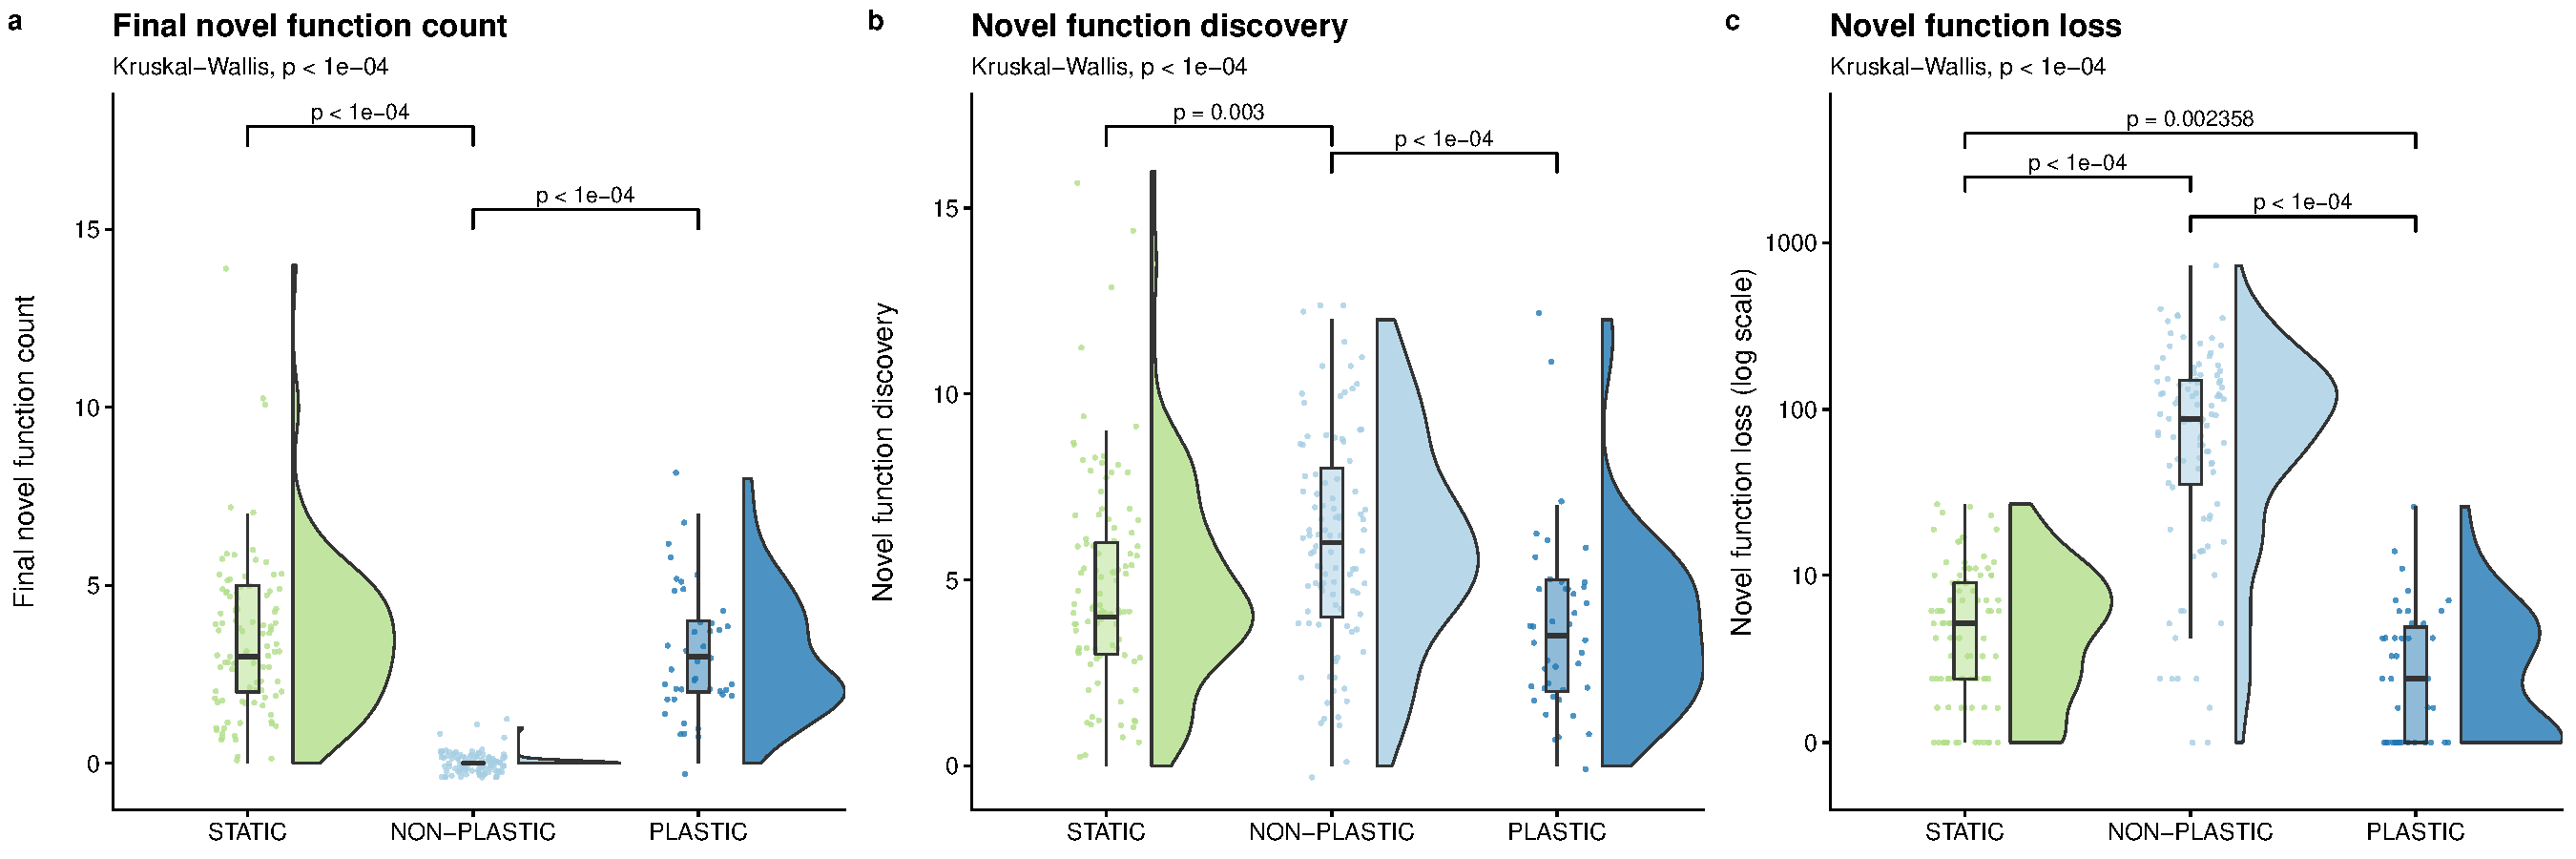
\includegraphics[width=0.9\textwidth]{media-complex-traits-magnitude-panel.pdf}
    \caption{\small
    \textbf{Novel task evolution.}
    Raincloud plots of
    (a) final novel task count,
    (b) novel task discovery,
    and (c) novel task loss.
    See Table \ref{tab:metrics-definitions} for descriptions of each metric.
    Each plot is annotated with statistically significant comparisons (Bonferroni-corrected pairwise Wilcoxon rank-sum tests).
    Note that adaptive phenotypic plasticity evolved in \novelTraitsPlasticReps\ of \novelTraitsReplicates\ replicates from the PLASTIC treatment during phase one of this experiment; we used this more limited group to seed the resulting \novelTraitsPlasticReps\ phase-two PLASTIC replicates.
    }
    \label{fig:complex-traits-magnitude}
\end{figure}

% -- What did we test? --
%In experimental phase 2B, we evaluated how evolution of adaptive phenotypic plasticity influences the ability of populations to evolve and retain novel adaptive traits. Commented out by Nkrumah...
We have so far shown that adaptive plasticity constrains the rate of evolutionary change in fluctuating environments.
However, it is unclear how this dynamic influences the evolution of novel tasks.
Based on their relative rates of evolutionary change, we might expect NON-PLASTIC-treatment populations to evolve more novel tasks than PLASTIC-treatment populations.
But, how much of the evolutionary change in NON-PLASTIC populations is useful for exploring novel regions of the fitness landscape versus continually rediscovering the same regions?

% - Magnitude of exploration/exploitation -
To answer this question, we quantified the number of novel tasks performed by a representative organism in the final population of each replicate.
We found that both PLASTIC and STATIC populations had significantly higher final task counts than NON-PLASTIC populations at the end of the experiment (Figure~\ref{fig:complex-traits-magnitude}a).
The final novel task count in PLASTIC and STATIC lineages could be higher than that of the NON-PLASTIC lineages for several non-mutually exclusive reasons.
One possibility is that PLASTIC and STATIC lineages could be exploring a larger area of the fitness landscape when compared to NON-PLASTIC lineages.
Another possibility is that the propensity of the NON-PLASTIC lineages to maintain novel traits could be significantly lower than PLASTIC or STATIC lineages.
When we looked at the total sum of novel tasks discovered by each of the PLASTIC, STATIC, and NON-PLASTIC lineages, we found that NON-PLASTIC lineages generally explored a larger area of the fitness landscape (Figure~\ref{fig:complex-traits-magnitude}b).
Although the NON-PLASTIC lineages discovered more novel tasks, those lineages also exhibited significantly higher novel task loss when compared to PLASTIC and STATIC lineages (Figure~\ref{fig:complex-traits-magnitude}c).

\begin{figure}[h!]
    \centering
    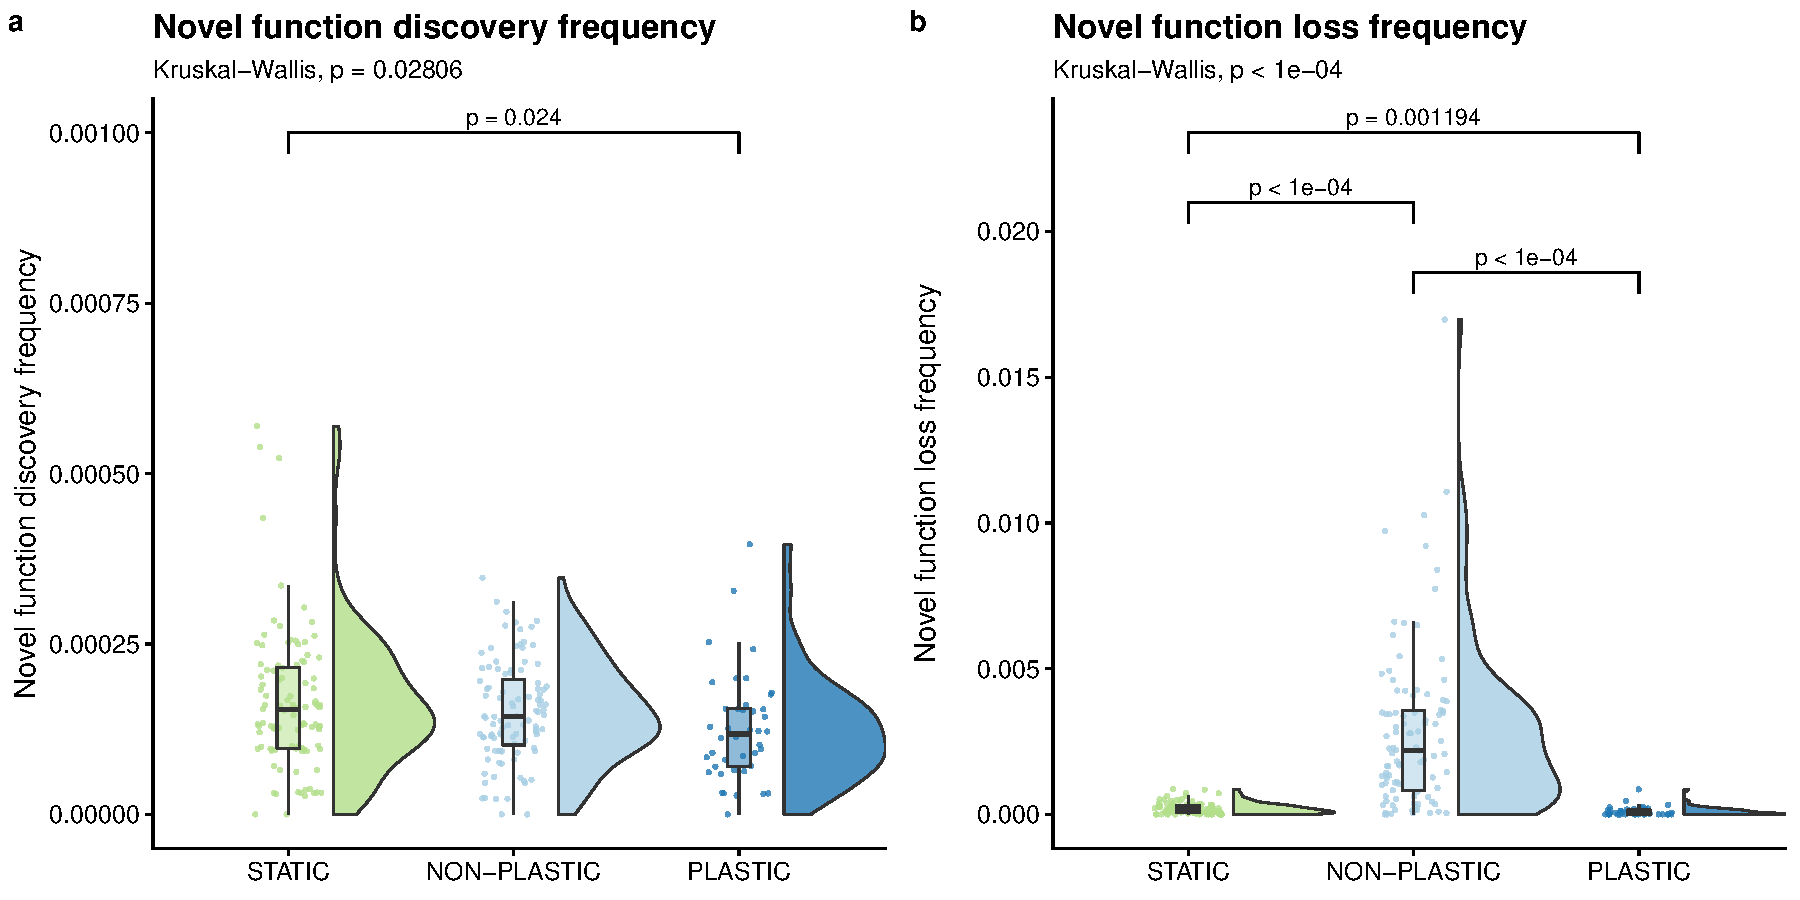
\includegraphics[width=0.66\textwidth]{media-complex-traits-pace-panel.pdf}
    \caption{\small
    \textbf{Rate of novel task evolution.}
    Raincloud plots of
    (a) novel task discovery frequency
    and (b) novel task loss frequency.
    Each plot is annotated with statistically significant comparisons (Bonferroni-corrected pairwise Wilcoxon rank-sum tests).
    }
    \label{fig:complex-traits-rate}
\end{figure}

% - Rates of exploration/exploitation -
A larger number of generations elapsed in NON-PLASTIC populations than in PLASTIC or STATIC populations during our experiment \citep{supplemental_material}.
Are NON-PLASTIC lineages discovering and losing novel tasks more frequently than PLASTIC or STATIC lineages, or are our observations a result of differences in generational turnover?
To answer this question, we converted the metrics of novel task discovery and novel task loss to rates by dividing each metric by the number of elapsed generations along the associated representative lineages.
We found no significant difference in the frequency of novel task discovery between NON-PLASTIC and STATIC lineages, and we found that PLASTIC lineages had a lower frequency of novel task discovery than STATIC lineages (Figure~\ref{fig:complex-traits-rate}a).
Therefore, we cannot reject the possibility that the larger magnitude of task discovery in NON-PLASTIC lineages was driven by a larger number of elapsed generations.
NON-PLASTIC lineages had a higher frequency of task loss than either PLASTIC or STATIC lineages, and PLASTIC lineages tended to have a lower frequency of novel task loss than STATIC lineages (Figure~\ref{fig:complex-traits-rate}b).


% - Characterizing trait loss -
Next, we examined the frequency at which novel task loss along lineages co-occurred with the loss or gain of any of the six base tasks.
Across all NON-PLASTIC representative lineages, over 97\% (10998 out of 11229) of instances of novel task loss co-occurred with a simultaneous change in base task profile.
In contrast, across all PLASTIC and STATIC dominant lineages, we observed that approximately 20\% (29 out of 142) and 2\% (13 out of 631), respectively, of instances of novel task loss co-occurred with a simultaneous change in base task profile.
As such, the losses of novel tasks in NON-PLASTIC lineages appear to be primarily due to hitchhiking.

\subsection{Lineages without plasticity that evolve in fluctuating environments express more deleterious tasks}

%%%%%%
% 2021-02-05 - Results
% - Number of offspring on lineage where hitchhiker instruction execution increases (i.e., instances of hitchhiking)
%   - PLASTIC ~~ STATIC < NON-PLASTIC
% - Hitchhiker instruction increases / offspring on lineage
%   - PLASTIC ~~ STATIC < NON-PLASTIC
% - What fraction of mutations that increase hitchhiker instruction execution co-occur with base trait changes?
%   - NON-PLASTIC > PLASTIC ~~ STATIC
% - What about unexpressed vs expressed trait changes in plastic populations? (plastic only)
%   - Not much hitchhiking. Did not find evidence that hitchiking occurring as cryptic variation in unexpressed phenotype.
%%%%%%

Phenotypic plasticity allows for genetic variation to accumulate in genomic regions that are unexpressed, which could lead to the fixation of deleterious instructions in PLASTIC populations.
However, in NON-PLASTIC lineages, we observe a higher rate of novel task loss, indicating that they may be more susceptible to deleterious mutations (Figure \ref{fig:complex-traits-rate}b).

Therefore, in experiment phase 2C, we tested whether adaptive phenotypic plasticity can increase the incidence of deleterious task performance.
Specifically, we added an instruction that triggered a ``poisonous'' task and measured the number of times it was executed.
Each execution of the  \code{poison} instruction reduces an organism's fitness by 10\%.
At the beginning of phase 2C, the \code{poison} instruction is not present in the population, as it was not part of the instruction set during phase one of evolution.
Accordingly, if a \code{poison} instruction fixes in a population, it must be the result of evolutionary dynamics during phase 2C, including cryptic variation or hitchhiking.

\begin{figure}[ht!]
    \centering
    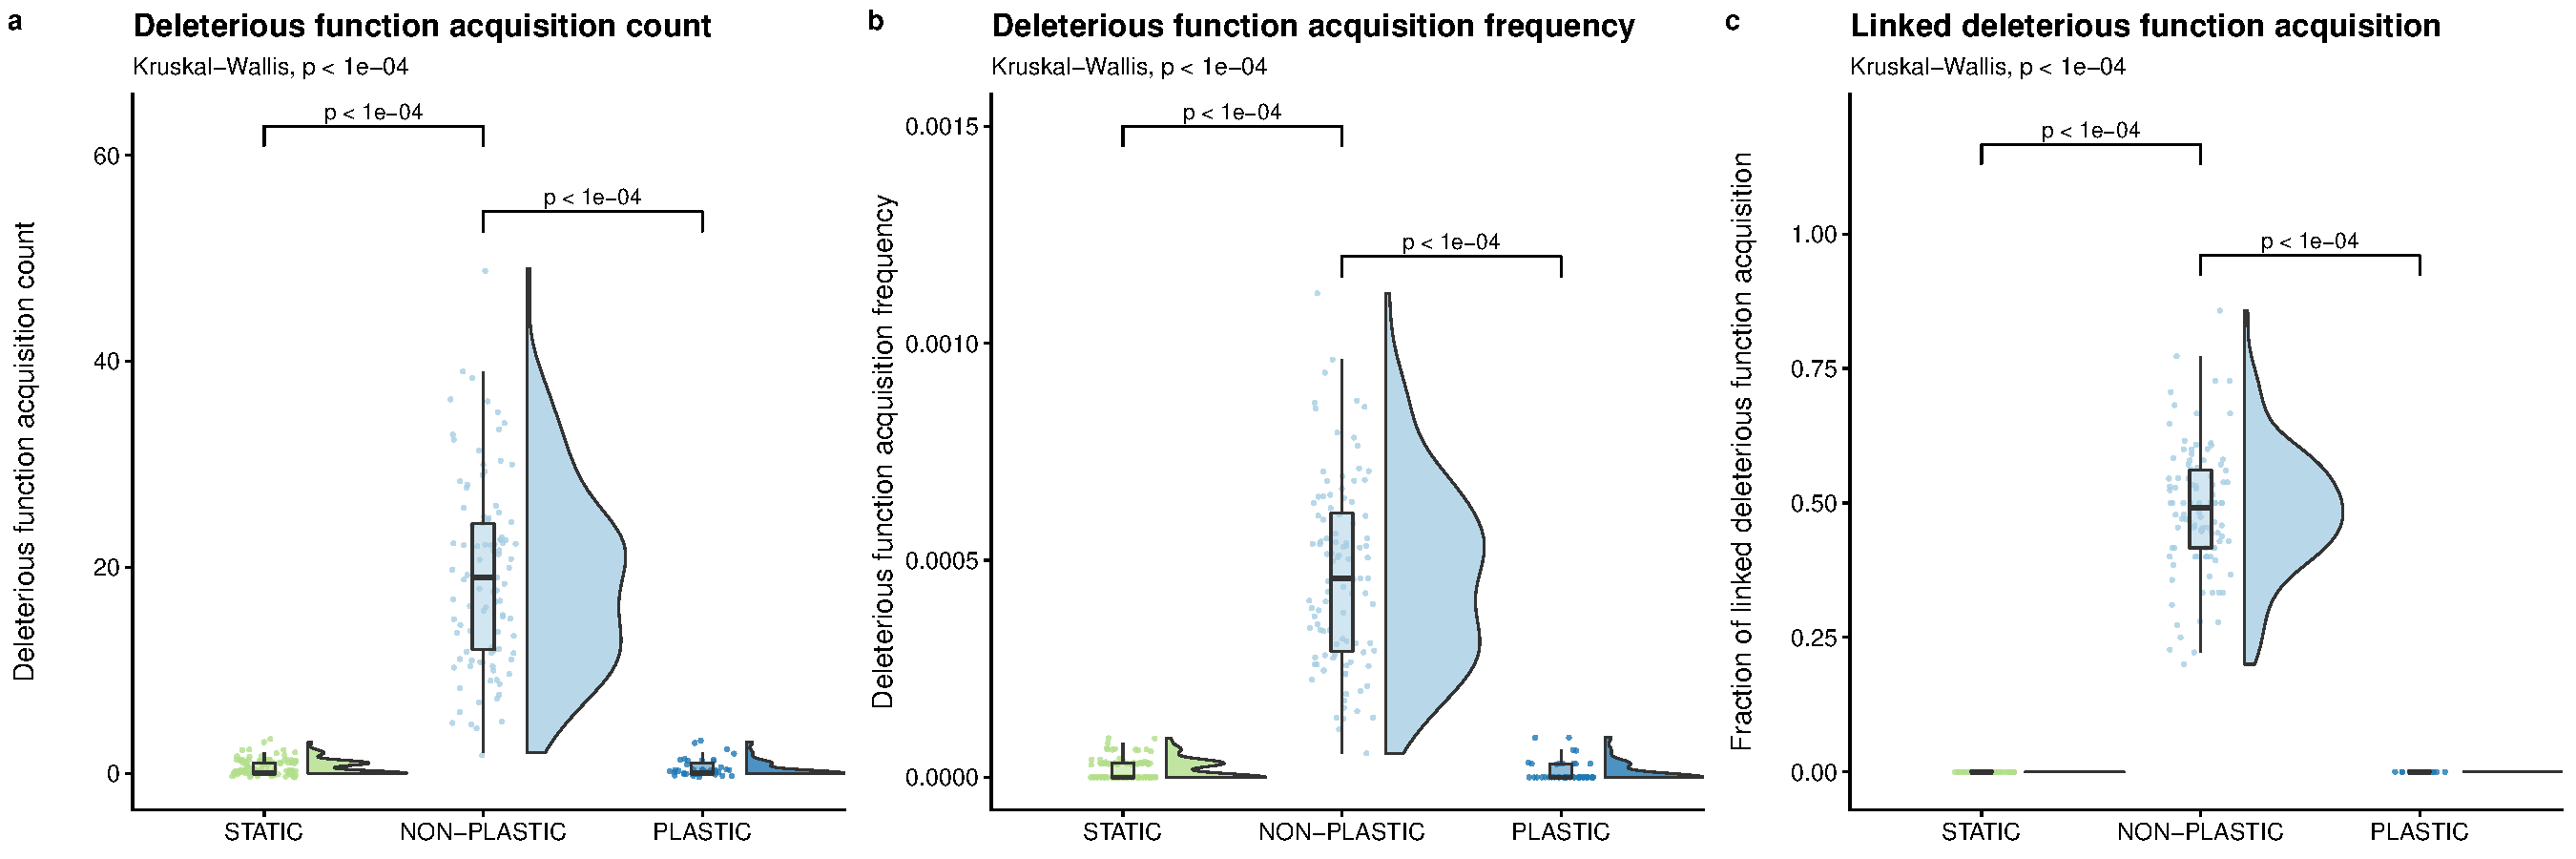
\includegraphics[width=1.0\textwidth]{media-poison-accumulation-panel.pdf}
    \caption{\small
    \textbf{Deleterious instruction accumulation.}
    Raincloud plots of
    (a) poisonous task acquisition,
    (b) poisonous task acquisition frequency,
    and (c) the proportion of mutations that increase poisonous task performance along a lineage that co-occur with a change in phenotypic profile.
    Each plot is annotated with statistically significant comparisons (Bonferroni-corrected pairwise Wilcoxon rank-sum tests).
    Note that adaptive phenotypic plasticity evolved in \deleteriousHitchhikingPlasticReps\ of \deleteriousHitchhikingReplicates\ replicates from the PLASTIC treatment during phase one of this experiment; we used this more limited group to seed the \deleteriousHitchhikingPlasticReps\ phase-two PLASTIC replicates.
    }
    \label{fig:deleterious-hitchhiking}
\end{figure}

% -- Instruction execution by final dominant & along lineage --
At the end of our experiment, no representative organisms from the PLASTIC or STATIC treatments performed the poisonous task under any environmental condition; however, representative organisms in 14\% of replicates of the NON-PLASTIC treatment performed the poisonous task at least once.
NON-PLASTIC lineages contained significantly more mutations that conferred the poisonous task as compared to PLASTIC or STATIC lineages (Figure \ref{fig:deleterious-hitchhiking}a), and these mutations occurred at a significantly higher frequency in NON-PLASTIC lineages (Figure \ref{fig:deleterious-hitchhiking}b).
% Additionally, we did not observe
% This result does not change when we normalize [what?] by the number of generations represented in the given lineage (Figure \ref{fig:deleterious-hitchhiking}b).

% -- When/where does hitchhiking take place? --
Next, we measured how often mutations that increased poisonous task performance co-occurred with changes to the base task profile within representative lineages.
A poisonous instruction can fix in a lineage by having a beneficial effect that outweighs its inherent cost (\textit{e.g.}, knocking out a punished task) or through linkage with a secondary beneficial mutation at another site within the genome.
Across all NON-PLASTIC representative lineages, we found that approximately 49\% (956 out of 1916) of mutations that increased poisonous task expression co-occurred with a change in the base task profile (Figure \ref{fig:deleterious-hitchhiking}c).
In all representative lineages from the PLASTIC treatment, only 18 mutations increased poisonous task expression, and none co-occurred with a change in base task profile (Figure \ref{fig:deleterious-hitchhiking}c).
Likewise, only 58 mutations increased poisonous task performance in all representative lineages from the STATIC treatment, and none co-occurred with a change in base task profile (Figure \ref{fig:deleterious-hitchhiking}c).
We did not find compelling evidence that the few mutations that increased poisonous task expression occurred as cryptic variation in PLASTIC lineages.

We repeated this experiment with 3\% and 30\% metabolic rate penalties associated with the poisonous task, which produced results that were consistent with those reported here \citep{supplemental_material}.

% GUIDELINES:
% This section may be divided by subheadings. Discussions should cover the key findings of the study: discuss any prior research related to the subject to place the novelty of the discovery in the appropriate context, discuss the potential shortcomings and limitations on their interpretations, discuss their integration into the current understanding of the problem and how this advances the current views, speculate on the future direction of the research, and freely postulate theories that could be tested in the future.

\section{Discussion}

In this work, we used evolving populations of digital organisms to determine how adaptive phenotypic plasticity alters subsequent evolutionary dynamics and influences evolutionary outcomes in fluctuating environments.
Specifically, we compared lineages of adaptively plastic organisms in fluctuating environments to both non-plastic organisms in those same environments and other non-plastic organisms in static environments.

\subsection{Evolutionary change}

% -- Adaptively plastic populations underwent less evolutionary change than non-plastic populations --
We found strong evidence that adaptive plasticity slows evolutionary change in fluctuating environments. 
Adaptively plastic populations experienced fewer coalescence events and fewer total genetic changes relative to non-plastic populations evolving under identical environmental conditions (Figure \ref{fig:evolutionary-dynamics-magnitude}).
Whereas non-plastic populations relied on \textit{de novo} mutations to adapt to each environmental fluctuation, plastic populations leveraged sensory instructions to regulate task performance. 
Indeed, in fluctuating environments, selection pressures toggle after each environmental change.
We hypothesize that in non-plastic populations such toggling would repeatedly drive the fixation of mutations that align an organism's phenotypic profile to the new conditions.
This hypothesis is supported by the increased frequency of coalescence events in these populations (Figure \ref{fig:evolutionary-dynamics-rate}a) as well as increased rates of genetic and phenotypic changes observed along the lineages of non-plastic organisms. 


%TODO: Make sure we use org vs. genotype consistently with rest of paper
% - Mutational neighborhood results
%We expected this was [caused by / due to / the result of] non-plastic populations evolving a bet-hedging strategy where mutations are more likely to modify the phenotypic profile.
%However, when we repeated the mutational robustness analysis on the mutational neighborhoods of representative genotypes (\textit{i.e.}, all possible one-step mutants), across the three conditions we observed the highest mutational robustness in the non-plastic condition (Figure \ref{fig:neighborhood-mutational-stability}).
Representative lineages in the non-plastic treatment experienced lower realized mutational robustness than plastic and static lineages (Figure \ref{fig:evolutionary-dynamics-rate}b).
We reasoned that this lower realized mutational robustness was due to non-plastic populations evolving a bet-hedging strategy where mutations are more likely to modify the phenotypic profile. 
However, when we switched from measuring the realized mutational robustness of representative lineages to measuring the mutational robustness of representative genotypes (\textit{i.e.}, what fraction of one-step mutants change the phenotypic profile), we observed that non-plastic genotypes exhibited the highest mutational robustness of all three treatments (Figure \ref{fig:mutational-robustness}).
This result runs contrary to both our expectations and the results of other fluctuating environment studies in Avida \citep{canino-koning_fluctuating_2019}.
\cite{canino-koning_fluctuating_2019} found that mutational robustness is negatively correlated with the number of task-encoding sites in the genome.
In our work, most plastic and static genotypes encode all six base tasks, while most non-plastic genotypes only encode tasks from one environment; this results in fewer task-encoding sites, which may increase mutational robustness in non-plastic genotypes (relative to plastic and static genotypes). %relative to genotypes from other treatments. 
Regardless of the cause, this higher mutational robustness in non-plastic organisms indicates that bet-hedging is not driving the low realized mutational robustness observed in non-plastic lineages.
Thus, we expect the lower realized mutational robustness in non-plastic lineages to be driven by survivorship bias. 
%Because non-plastic lineages must rely on mutations to adapt to environmental changes, these adaptive mutations are highly beneficial and are thus selected. 
%This decreases the realized mutational robustness of the lineage even though
Because non-plastic lineages must rely on mutations to adapt to environmental changes, phenotype-altering mutations are often highly advantageous, and their selection decreases the realized mutational robustness of the lineage. 
%We expect this result to thus be due to survivorship bias, as non-plastic lineages rely on mutations to adapt to their environment, and thus the phenotype-changing mutations that do occur are highly adaptive and thus selected. 
%Future work is needed to determine if there are other contributing factors. 


% -- in context of previous digital evolution work --
To our knowledge, this study is the first in-depth empirical investigation into how the \textit{de novo} evolution of adaptive plasticity shifts the course of subsequent evolution in a cyclic environment.
The relative rates of evolutionary change that we observed in non-plastic populations, however, are consistent with results from previous digital evolution studies. 
For example, \cite{dolson_interpreting_2020} showed that non-plastic populations that were evolved in cyclically changing environments exhibited higher phenotypic volatility and accumulated more mutations than that of populations evolved under static conditions.
Furthermore, \cite{lalejini_evolutionary_2016} visually inspected the evolutionary histories of non-plastic organisms evolved in fluctuating environments, observing that mutations along successful lineages readily switched the set of traits expressed by offspring.
%\cite{canino-koning_evolution_2016} also observed that genomes evolved in harsh cyclic environments often contained vestigial fragments of genetic material adapted to prior environments.


% -- In context of conventional evolutionary theory: evo response => f(selection, variation) --
Our results are also consistent with conventional evolutionary theory.
A trait's evolutionary response to selection depends on the strength of directional selection and on the amount of genetic variation for selection to act upon \citep{lande_measurement_1983,zimmer_evolution_2013}.
In our experiments, non-plastic populations repeatedly experienced strong directional selection to toggle which tasks were expressed after each environmental change.
As such, retrospective analyses of successful lineages revealed rapid evolutionary responses (that is, high rates of genetic and phenotypic changes).
Evolved adaptive plasticity shielded populations from strong directional selection when the environment changed by eliminating the need for a rapid evolutionary response to toggle task expression.
Indeed, both theoretical and empirical studies have shown that adaptive plasticity can constrain evolutionary change by weakening directional selection on evolving populations \citep{price_role_2003,paenke_influence_2007,ghalambor_non-adaptive_2015}. 

% TODO, consider: Expectations that could arise if we took into consideration lineages off the line of descent. 

% \vspace{0.25cm}
\subsection{The evolution and maintenance of novel tasks}

% -- Exploration + Exploitation --
In fluctuating environments, non-plastic populations explored a larger area of the fitness landscape than adaptively plastic populations (Figure \ref{fig:complex-traits-magnitude}b).
However, adaptively plastic populations better exploited the fitness landscape, retaining a greater number of novel tasks than non-plastic populations evolving under identical environmental conditions (Figure \ref{fig:complex-traits-magnitude}a).
In our experiment, novel tasks were less important to survival than the fluctuating base tasks.
In non-plastic populations, when a mutation changes a base task to better align with current environmental conditions, its benefit will often outweigh the cost of losing one or more novel tasks. 
%Indeed, we found that mutations associated with novel task loss along representative lineages from non-plastic populations co-occurred with phenotypic changes that helped offspring adapt to current environmental conditions 97\% of the time.
Indeed, we found that along non-plastic representative lineages, 97\% of the mutations associated with novel task loss co-occurred with phenotypic changes that helped offspring adapt to current environmental conditions. 

% -- Changing environments promote evolutionary change --
Previous studies have shown that transitory environmental changes can improve overall fitness landscape exploration in evolving populations of non-plastic digital organisms \citep{nahum_improved_2017}.
Similarly, changing environments have been shown to increase the rate of evolutionary adaptation in simulated network models \citep{kashtan2007varying}.
In our system, however, we found that \textit{repeated} fluctuations reduced the ability of non-plastic populations to maintain and exploit tasks; that said, we did find that repeated fluctuations may improve overall task discovery by increasing generational turnover. 
Consistent with our findings, \cite{canino-koning_fluctuating_2019} found that non-plastic populations of digital organisms evolving in a cyclic environment maintained fewer novel traits than populations evolving in static environments.

% -- Plastic rescue, stabilizing effect of plasticity --
Our results suggest that adaptive phenotypic plasticity can improve the potential for populations to exploit novel resources by stabilizing them against stressful environmental changes.
The stability that we observe may also lend some support to the hypothesis that phenotypic plasticity can rescue populations from extinction under changing environmental conditions \citep{chevin_adaptation_2010}.

% -- relevance to genes as followers hypothesis --.
Our data do not necessarily provide evidence for or against the genes as followers hypothesis.
The genes as followers hypothesis focuses on contexts where plastic populations experience novel or abnormally stressful environmental change.
However, in our system, environmental changes were cyclic (not novel), and no single environmental change was \textit{abnormally} stressful.
Further, the introduction of novel tasks during the second phase of the experiment merely added static opportunities for fitness improvement.
This addition did not change the meaning of existing environmental cues, nor did it require those cues to be used in new ways. 
 

% \vspace{0.25cm}
\subsection{The accumulation of deleterious alleles}

% -- Overview of results --
%   - More accumulation in non-plastic
%   - no evidence for cryptic variation housing poison
%   - plastic ~~ static
We found that non-plastic lineages that evolved in a fluctuating environment exhibited both greater totals and higher rates of poisonous task acquisition than that of adaptively plastic lineages (Figure \ref{fig:deleterious-hitchhiking}).
In asexual populations without horizontal gene transfer, all co-occurring mutations are linked.
As such, deleterious mutations linked with a stronger beneficial mutation (\textit{i.e.}, a driver) can sometimes ``hitchhike'' to fixation \citep{smith_hitch-hiking_1974,van_den_bergh_experimental_2018,buskirk_hitchhiking_2017}.
Natural selection normally prevents deleterious mutations from reaching high frequencies, as such mutants are outcompeted.
However, when a beneficial mutation sweeps to fixation in a clonal population, it carries along any linked genetic material, including other beneficial, neutral, or deleterious mutations \citep{barton_genetic_2000, smith_hitch-hiking_1974}.
Therefore, we hypothesize that deleterious genetic hitchhiking drove \code{poison} instruction accumulation along non-plastic lineages in changing environments.

Across our experiments, the frequency of selective sweeps in non-plastic populations provided additional opportunities for genetic hitchhiking with each environmental change. 
Indeed, representative lineages from non-plastic populations in the cyclic environment exhibited higher mutation accumulation (Figure~\ref{fig:evolutionary-dynamics-magnitude}b), novel trait loss (Figure~\ref{fig:complex-traits-magnitude}c), and poisonous task acquisition (Figure~\ref{fig:deleterious-hitchhiking}a) than their plastic counterparts.
In aggregate, we found that many ($\sim$49\%; 956 / 1916) mutations that increased \code{poison} instruction execution in offspring co-occurred with mutations that provided an even stronger benefit by adapting the offspring to an environmental change.
We expect that an even larger fraction of these deleterious mutations were linked to beneficial mutations, but our analysis only counted mutations that co-occurred in the same generation.


% -- Elaboration on plastic result --
Theory predicts that under relaxed selection deleterious mutations should accumulate as cryptic variation in unexpressed traits \citep{lahti_relaxed_2009}.
Contrary to this expectation, we did not find evidence of \code{poison} instructions accumulating as cryptic variation in adaptively plastic lineages.
One possible explanation is that the period of time between environmental changes was too brief for variants carrying unexpressed \code{poison} instructions to drift to high frequencies before the environment changed, after which purifying selection would have removed such variants.
Indeed, we would not expect drift to fix an unexpressed trait since we tuned the frequency of environmental fluctuations to prevent valuable traits from being randomly eliminated during the off environment.
Additionally, plastic organisms in Avida usually adjust their phenotype by toggling the expression of a minimal number of key instructions, leaving little genomic space for cryptic variation to accumulate.

\subsection{Limitations and future directions}

% ------------
% Possible additional future directions:
% - Need to look at mutations off the line of descent 
% - Variable length genomes
% - Relaxed selection, mutational decay
% ------------

% -- Adaptive vs non-adaptive plasticity --
Our work lays the groundwork for using digital evolution experiments to investigate the evolutionary consequences of phenotypic plasticity in a range of contexts.
However, the data presented here are limited to the evolution of \textit{adaptively} plastic populations.
Future work might explore the evolutionary consequences of maladaptive and non-adaptive phenotypic plasticity (\textit{e.g.}, \citealt{leroi_temperature_1994}), which are known to bias evolutionary outcomes \citep{ghalambor_non-adaptive_2015}. 
% -- Environmental change --
Additionally in our experiments, sensory instructions perfectly differentiated between ENV-A and ENV-B, and environmental fluctuations never exposed populations to entirely new conditions.
These parameters have been shown to influence evolutionary outcomes \citep{li_digital_2004,boyer_adaptation_2021}, which if relaxed in the context of further digital evolution experiments, may yield additional insights.

% - limitation: focus on lineages -
%   - extend to complete evolutionary histories
We focused our analyses on the lineages of organisms with the most abundant genotype in the final population.
These successful lineages represented the majority of the evolutionary histories of populations at the end of our experiment, as populations did not exhibit long-term coexistence of different clades.
Our analyses, therefore, gave us an accurate picture of what fixed in the population.
We did not, however, examine the lineages of extinct clades.
Future work will extend our analyses to include extinct lineages, giving us a more complete view of evolutionary history, which may allow us to better distinguish adaptively plastic populations from populations evolving in a static environment. 

% - Machinery -
As with any wet-lab experiment, our results are in the context of a particular model organism: ``Avidian'' self-replicating computer programs.
Digital organisms in Avida regulate responses to environmental cues using a combination of sensory instructions and conditional logic instructions (\code{if} statements).
The \code{if} instructions conditionally execute a single instruction depending on previous computations and the state of memory. 
As such, plastic organisms in Avida typically regulate phenotypes by toggling the expression of a small number of key instructions as opposed to regulating cohorts of instructions under the control of a single regulatory sequence \citep{supplemental_material}. 
This bias may limit the accumulation of hidden genetic variation in Avida genomes. 
However, as there are many model biological organisms, there are many model digital organisms that have different regulatory mechanisms (\textit{e.g.}, \citealt{lalejini_evolving_2018}) that should be used to test the generality of our results.

% [A broad sentence to wrap everything up?]
% e.g., A sentence about how we hope this work inspires more use of digital evolution as an experimental tool/expand experimental repertoire of evolutionary biologists studying phenotypic plasticity?
% e.g., As demonstrated here, Digital evolution studies allow us to directly manipulate the capacity for plastic responses to evolve and perfectly observe subsequent dynamics, enabling us to experimentally test hypotheses that were previously relegated to theoretical analyses.



\end{raggedbottom}


% \href{http://home.frontiersin.org/about/author-guidelines#SupplementaryMaterial}{Supplementary Material} should be uploaded separately on submission, if there are Supplementary Figures, please include the caption in the same file as the figure. LaTeX Supplementary Material templates can be found in the Frontiers LaTeX folder.

\section*{Supplemental Material}

The supplemental material for this article is hosted on GitHub and can be found online at \url{https://github.com/amlalejini/evolutionary-consequences-of-plasticity} \citep{supplemental_material}.
 

% Please see the availability of data guidelines for more information, at https://www.frontiersin.org/about/author-guidelines#AvailabilityofData
% The datasets [GENERATED/ANALYZED] for this study can be found in the [NAME OF REPOSITORY] [LINK].

\section*{Data Availability Statement}

The datasets generated and analyzed for this study can be found on the Open Science Framework at \url{https://osf.io/sav2c/} \citep{osf_data}.



% The Author Contributions section is mandatory for all articles, including articles by sole authors. If an appropriate statement is not provided on submission, a standard one will be inserted during the production process. The Author Contributions statement must describe the contributions of individual authors referred to by their initials and, in doing so, all authors agree to be accountable for the content of the work. Please see  \href{http://home.frontiersin.org/about/author-guidelines#AuthorandContributors}{here} for full authorship criteria.

\section*{Author Contributions}

AL and AJF designed the experiments, developed the necessary experiment software, conducted experiments, analyzed the results, and drafted the manuscript. 
AL, AJF, NAG and CO edited and approved the manuscript. 


% Details of all funding sources should be provided, including grant numbers if applicable. Please ensure to add all necessary funding information, as after publication this is no longer possible.

\section*{Funding}

% This work was supported by funding from TODO
% AL: Michigan State University (UDF), DGE-1424871
% AJF: U.S. National Science Foundation grant DEB-1655715 (Should check with Charles to make sure)
% NG DE-SC0019436 Department of Energy
% CO

This research was supported by the Department of Energy through Grant No. DE-SC0019436 and by the National Science Foundation (NSF) through the BEACON Center (DBI-0939454), a Graduate Research Fellowship to AL (DGE-1424871), and NSF Grant No. DEB-1655715. 

%  to CO (which supported AJF)



% All financial, commercial or other relationships that might be perceived by the academic community as representing a potential conflict of interest must be disclosed. If no such relationship exists, authors will be asked to confirm the following statement: 
% "The authors declare that the research was conducted in the absence of any commercial or financial relationships that could be construed as a potential conflict of interest."

\section*{Conflict of Interest Statement}

The authors declare that the research was conducted in the absence of any commercial or financial relationships that could be construed as a potential conflict of interest.

% This is a short text to acknowledge the contributions of specific colleagues, institutions, or agencies that aided the efforts of the authors.

\section*{Acknowledgments}

% Preliminary experiments from which this work sprouted, ALife 2020 keynote

We thank members of the MSU Digital Evolution Lab for helpful comments and suggestions on this work. 
We also thank Luis Zaman whose keynote talk at the 2020 Artificial Life conference inspired the initial exploratory experiments from which this work blossomed. 
MSU provided computational resources through the Institute for Cyber-Enabled Research. 
Any opinions, findings, and conclusions or recommendations expressed in this material are those of the author(s) and do not necessarily reflect the views of the National Science Foundation, Department of Energy, Michigan State University, or The University of Idaho.

\bibliographystyle{frontiersinSCNS_ENG_HUMS}
\bibliography{references,software}

\end{document}
